\documentclass{AeroStructure-ERJohnson}
\input crosslink.tex

%\usepackage{showframe}
\def\ShowFrameLinethickness{0.125pt}

\def\harp#1{\smash{\mathord{\buildrel{\lower3pt\hbox{$\scriptscriptstyle\rightharpoonup$}}\over{#1}}}}

\myexternaldocument{App_4P}
\myexternaldocument{Ch01_4P}
\myexternaldocument{Ch02_4P}
\myexternaldocument{Ch03_4P}
\myexternaldocument{Ch04_4P}
\myexternaldocument{Ch05_4P}
\myexternaldocument{Ch06_4P}
%\myexternaldocument{Ch07_4P}
\myexternaldocument{Ch08_4P}
\myexternaldocument{Ch09_4P}
\myexternaldocument{Ch10_4P}
\myexternaldocument{Ch11_4P}
\myexternaldocument{Ch12_4P}
\myexternaldocument{Ch13_4P}
\myexternaldocument{Ch14_4P}
\myexternaldocument{Ch15_4P}
\myexternaldocument{Ch16_4P}
\myexternaldocument{Ch17_4P}
\myexternaldocument{Ch18_4P}

\setcounter{chapter}{6}

\begin{document}

\mainmatter

%\hbox{~}\clearpage
\setcounter{page}{175}

\setcounter{chapter}{6}

\chapter{Arches, rings and fuselage frames} \label{ch7}

A common structural component in aerospace structures is a curved bar. For example, fuselage frames are often composed of slender curved elements and thin rings. The Winkler\footnote{Emil Winkler, 1835--1888, German civil engineer and professor.} theory for the linear elastic response of co-planar curved bars within their plane is presented in article~\ref{sec7.1}. (Also refer to Langhaar, 1962). The Winkler theory models both thick and thin curved bars. A curved bar is generally considered thin if the ratio of the radius of curvature to its the in-plane thickness is greater than ten. Ratios less than ten are considered thick bars. It is assumed that there is no out-of-plane bending and torsion of the bar in article~\ref{sec7.1}. Consistent with this limitation and assumption is an idealization employed in aircraft structural analyses that a ring frame is coplanar structure supporting loads in its plane and not supporting loads normal to its plane. Out-of plane bending and torsion of planar, thin curved bars is reviewed in the article by Chidamparam and Leissa (1993).

\section{Coplanar curved bars}\label{sec7.1}

The reference axis of the bar is defined as a uniformly continuous plane curve within a closed interval. It is assumed that the cross sections of the bar are symmetric with respect to the plane of the reference axis, and that the locus of points along the centroids of each cross section coincide with the reference axis. Only deformations of the bar in the plane of symmetry are considered.

{\def\thefigure{7.1}
\processfigure{\includegraphics{Figure_7-1.pdf}
}{\caption{Geometry of a coplanar curved bar defined in its plane of symmetry.\label{fig7.1}}}}



The Cartesian coordinates of the reference axis with origin at point O are denoted by $y_{0}(s)$ and $z_{0}(s)$ in the plane of symmetry, where $s$ denotes the curvilinear coordinate of the reference axis. Geometry of the curved bar in its plane of symmetry is shown in figure~\ref{fig7.1}. The position vector of the reference axis with respect to the origin O is $\harp{r}(s)=y_{0}(s) \hat{j}_{0}+z_{0}(s) \hat{k}_{0}$, where $\hat{j}_{0}$ and $\hat{k}_{0}$ are fixed unit vectors along the positive $y_0$ and $z_0$ directions, respectively. The unit tangent vector to the reference axis at point $s$ is
\begin{align}\label{eq7.1}
\hat{t}(s)=\frac{d \harp{r}}{d s}=\frac{d y_{0}}{d s} \hat{j}_{0}+\frac{d z_{0}}{d s} \hat{k}_{0}.
\end{align}
The Cartesian coordinates in a cross section are denoted by $x$ and $y$ with origin at the centroid labeled C as is shown in section A-A of figure~\ref{fig7.1}. Let $\theta(s)$ denote the angle from the fixed unit vector $\hat{k}_{0}$ to the unit tangent vector $\hat{t}(s)$, and let $\hat{j}(s)$ denote the unit vector normal to reference axis at $s$. The positive $y$-coordinate is directed\break along the unit normal $\hat{j}(s)$. From the triangular insert in figure~\ref{fig7.1} we see that the differential Cartesian coordinates along the reference axis are related to the angle $\theta$ by $d y_{0}=(-\sin \theta) d s$ and $d z_{0}=(\cos \theta) d s$. Thus, the unit tangent vector $\hat{t}(s)$ and the unit normal vector $\hat{j}(s)$ to the reference axis at $s$ are given by
\begin{align}\label{eq7.2}
\hat{t}(s)=-\sin \theta(s) \hat{j_{0}}+\cos \theta(s) \hat{k_{0}} \quad \hat{j(s)}=\cos \theta(s) \hat{j_{0}}+\sin \theta(s) \hat{k_{0}}.
\end{align}
From the previous equation we obtain the derivatives of the unit tangent vector and unit normal vector with respect to arc-length as
\begin{align}\label{eq7.3}
\frac{d \hat{t}}{d s}=\frac{-\hat{j}}{R(s)} \quad \frac{d j}{d s}=\frac{\hat{t}}{R(s)} \quad \frac{1}{R(s)}=\frac{d \theta}{d s},
\end{align}
where $R(s)$ denotes the radius of curvature of the reference axis at $s$. A curve parallel to the reference axis is characterized by a fixed value of the $y$-coordinate. Let the position vector of a parallel curve with respect to origin O be denoted by $\harp{R}$, where $\harp{R}(s, y)=\hat{r}(s)+y \hat{j}(s)$. Then, the differential of this position vector along the parallel curve is $d \harp{R}=dS \hat{t}$, where $d S$ is the differential arc-length along the parallel curve. The differential arc-length of the parallel curve is related to the corresponding differential arc length of the reference axis by
\begin{align}\label{eq7.4}
d S=\left(1+\frac{y}{R(s)}\right) d s.
\end{align}

\subsection{Displacements and strain}\label{sec7.1.1}

Consider the displacement of a particle located by $\harp{R}(S, y)$ on the parallel curve to the position located by vector $\harp{R^{*}}\left(S^{*}, y\right)$ with respect to origin O on the parallel curve in the deformed bar. Let \textit{S}* denote the arc-length along the parallel curve in the deformed bar, where the $y$-coordinate remains unchanged in the deformation. That is, \textbf{it is assumed the cross section remains rigid in its own plane}. We write the position of the particle in the deformed bar with respect to its position in the undeformed bar as $\harp{R^{*}} =\harp{R}+\bar{u}$, where the displacement vector is defined by\vspace*{-3pt}
\begin{align}\label{eq7.5}
\harp{u}(S, y)=u_{s}(S, y) \hat{t}(s)+u_{y}(S, y) \hat{j}(s).
\end{align}
The differential of $\harp{R^{*}}\left(S^{*}, y\right)$ along the parallel curve in the deformed bar is given by\pagebreak
\begin{align}\label{eq7.6}
d \harp{R}^{*}=d S \hat{t}+\frac{d}{d S}\left(u_{s} \hat{t}+u_{y} j\right) d S=d S \hat{t}+\left[\frac{d}{d s}\left(u_{s} \hat{t}+u_{y} j\right)\right]\left(1+\frac{y}{R(s)}\right)^{-1} d S,
\end{align}
in which we use the chain rule of differentiation \Big(i.e., $\frac{d \harp{u}}{d S}=\frac{d \harp{u}}{d s} \frac{d s}{d S}$\Big) and eq.~(\ref{eq7.4}) to transform the derivative with respect \textit{S} to the derivative with respect s. Performing the differentiations in eq.~(\ref{eq7.6}) and using the relations in eq.~(\ref{eq7.3}), we get
\begin{align}\label{eq7.7}
d \harp{R}^{*}=\left[\hat{t}+\frac{1}{\left(1+\frac{y}{R}\right)} \frac{d}{d s}\left(u_{s} \hat{t}+u_{y} j\right)\right] d S=\left[\hat{t}+\frac{1}{\left(1+\frac{y}{R}\right)}\left[\left(\frac{d u_{s}}{d s}+\frac{u_{y}}{R}\right) \hat{t}+\left(\frac{d u_{y}}{d s}-\frac{u_{s}}{R}\right) \hat{j}\right]\right] d S.
\end{align}
The last result is written as\vspace*{-5pt}
\begin{align}\label{eq7.8}
d \harp{R^{*}}=[(1+\varepsilon) \hat{t}-\omega \hat{j}] d S,
\end{align}
where\vspace*{-5pt}
\begin{align}\label{eq7.9}
\varepsilon=\frac{R}{R+y}\left(\frac{d u_{s}}{d s}+\frac{u_{y}}{R}\right) \quad \omega=-\left(\frac{R}{R+y}\right)\left(\frac{d u_{y}}{d s}-\frac{u_{s}}{R}\right).
\end{align}



{\def\thefigure{7.2}
\processfigure[b]{\vspace*{-6pt}\includegraphics{Figure_7-2.pdf}
}{\caption{(a) Differential line element of a parallel curve in the deformed bar. (b) Relationship of
the displacement of a particle on a parallel curve to the displacement of the corresponding
particle on the reference axis.\label{fig7.2}}}}

The differential arc-length along the parallel curve in the deformed bar is determined by $\left(d S^{*}\right)^{2}=d \harp{R^{*}} \bullet d \harp{R^{*}}$, and the unit tangent vector to the parallel curve in the deformed bar is $\hat{t}^{*}=\left(d \harp{R^{*}}\right) /\left(d S^{*}\right)$. The stretch ratio $\lambda$ is defined by $d S^{*}=\lambda d S$, and with regard to eq.~(\ref{eq7.8}) $\lambda=\sqrt{(1+\varepsilon)^{2}+\omega^{2}}$. Consider the binomial series $\sqrt{1+\xi}=1+\xi / 2-\xi^{2} / 8 \pm \ldots.$ For $\xi=2 \varepsilon+\varepsilon^{2}+\omega^{2}$, the binomial series for the stretch ratio is $\lambda=1+\varepsilon+\omega^{2} / 2+\ldots.$ Since the engineering strain is defined by $\lambda-1=\varepsilon+\omega^{2} / 2+\ldots,$ we see that to the lowest degree in the series expansion of the engineering strain that $\varepsilon$ is interpreted as the normal strain of a parallel curve for infinitesimal deformation. To interpret the physical meaning of $\omega$ a graph of eq.~(\ref{eq7.8}) is shown in figure~\ref{fig7.2}(a). Let $\Omega$ denote the angle between the unit tangent vector $\hat{t}$ of the parallel curve in the undeformed bar and the unit tangent vector $\hat{t^{*}}$ of the parallel curve in the deformed bar. From the geometry of the triangle in figure~\ref{fig7.2}(a) we see that $\tan \Omega=\omega /(1+\varepsilon)$. Using the small angle approximation for the tangent function, and the assumption of infinitesimal strain, we find $\Omega \cong \omega$. That is, $\omega$ represents the rotation of the tangent line element to the parallel curve for infinitesimal deformations of the bar. Let $\hat{j}^{*}$ denote unit normal vector to $\hat{t^{*}}$. From figure~\ref{fig7.2}(a) the unit normal vector $\hat{j}^{*}=(\cos \Omega) \hat{j}+(\sin \Omega) \hat{t}$. For small angles $\Omega$, the unit normal vector approximates as
\begin{align}\label{eq7.10}
\hat{j}{ }^{*} \cong \hat{j}+\omega \hat{t}.
\end{align}
\noindent \textbf{The relationship between the displacement vector of the parallel curve to the displacement vector of the reference axis is based on the assumptions that plane cross sections normal to the reference axis remain normal to the reference axis in the deformed bar and that the cross section remains rigid in its own plane}. These assumptions, which are the basis of classical beam theory, are depicted in figure~\ref{fig7.2}(b). Thus,
\begin{align}\label{eq7.11}
\harp{u}(S, y)=\harp{u}_{C}(s)+y(\hat{j} * \hat{j}),
\end{align}
where the displacement vector of the reference axis is defined by
\begin{align}\label{eq7.12}
\harp{u}_{C}(s)=w(s) \hat{t}(s)+v(s) \hat{j}(s).
\end{align}
Substitute eq.~(\ref{eq7.5}) for $\harp{u}(S, y)$ in eq.~(\ref{eq7.11}), followed by substitutions of eq.~(\ref{eq7.10}) and (\ref{eq7.12}) into eq.~(\ref{eq7.11}) to find
\begin{align}\label{eq7.13}
u_{s}=w(s)+y \omega(s) \quad u_{y}=v(s).
\end{align}
Substitute the displacements of eq.~(\ref{eq7.13}) into the expression in eq.~(\ref{eq7.9}) for $\omega$ to get
\begin{align}\label{eq7.14}
\omega=-\left(\frac{R}{R+y}\right)\left(\frac{d v}{d s}-\frac{w(s)+y \omega}{R}\right)=-\left(\frac{R}{R+y}\right)\left(\frac{d v}{d s}-\frac{w(s)}{R}\right)+\frac{y \omega}{R+y}.
\end{align}
Solve eq.~(\ref{eq7.14}) for $\omega$ to find
\begin{align}\label{eq7.15}
\omega=-\left(\frac{d v}{d s}-\frac{w}{R}\right).
\end{align}
Finally, substitute the displacements of eq.~(\ref{eq7.13}) into the expression for $\varepsilon$ in eq.~(\ref{eq7.9}), followed by the substitution of $\omega$ from eq.~(\ref{eq7.15}), to get the strain-displacement relation for the curved bar as
\begin{align}\label{eq7.16}
\varepsilon=\frac{d w}{d s}+\frac{v}{R+y}-\frac{y}{R+y}\left[R\left(\frac{d^{2} v}{d s^{2}}\right)+\frac{w}{R}\left(\frac{d R}{d s}\right)\right].
\end{align}
Although the displacements (\ref{eq7.13}) are linear in the thickness coordinate $y$, note that the strain (\ref{eq7.16}) is non\-linear~in~$y$.

\subsection{Normal stress, stress resultants, and strain energy}\label{sec7.1.2}

The material of the bar is assumed to linear elastic, isotropic, and homogeneous. Then, the normal stress $\sigma$ acting on the cross section is related to the normal strain $\varepsilon$ via Hooke's law. As was discussed in article~\ref{sec3.7} we take $\sigma=E \varepsilon$, where \textit{E} is the modulus of elasticity of the material. The result for the normal stress is written as
\begin{align}\label{eq7.17}
\sigma=\frac{E}{R+y}\left\{\left(v+R \frac{d w}{d s}\right)+y\left[\frac{d w}{d s}-\left[R\left(\frac{d^{2} v}{d s^{2}}\right)+\frac{w}{R}\left(\frac{d R}{d s}\right)\right]\right]\right\}.
\end{align}
The normal force \textit{N} and bending moment \textit{M} about the centroidal $x$-axis of the cross section are related to the normal stress by\vspace*{-6pt}
\begin{align}\label{eq7.18}
(N, M)=\int_{A}(1, y) \sigma d A,
\end{align}
where \textit{A} denotes the cross-sectional area of the bar. Substitute Hooke's law for the normal stress (\ref{eq7.17}) into eq.~(\ref{eq7.18}) to get the relation between the resultants and the displacements. In this substitution process the following integrals over the cross section occur:
\begin{align}\label{eq7.19}
\int_{A} \frac{d A}{R+y}=\frac{A}{R}(1+Y) \quad \int_{A} \frac{y d A}{R+y}=-Y A \quad \int_{A} \frac{y^{2} d A}{R+y}=Y A R,
\end{align}
\vspace*{5pt}
\clearpage

\noindent in which \textit{Y} is the dimensionless parameter of Winkler's curved bar theory. Equivalence of the three integrals\break (\ref{eq7.19}) with respect to parameter \textit{Y} can be demonstrated by dividing the denominator into the numerator of the integrand in the first two integrals and noting $\int_A y d A=0$, since $y$ is measured from the centroid. Langhaar (1962) states that the third expression in eq.~(\ref{eq7.19}) is the most convenient for the evaluation of the parameter \textit{Y }if numerical integration is required. If $R \gg y$, then the third expression in eq.~(\ref{eq7.19}) approximates \textit{Y} as
\begin{align}\label{eq7.20}
Y \cong Y_{\mathrm{appx}}=I /\left(A R^{2}\right) \quad \text { where } \quad I=\int_{A} y^{2} d A.
\end{align}

\vspace*{-\baselineskip}
\noindent The equations for the resultants are\vspace*{-3pt}
\begin{gather}\label{eq7.21}
N=\frac{E A}{R}\left\{\left(v+R \frac{d w}{d s}\right)+Y\left[v+R\left[R\left(\frac{d^{2} v}{d s^{2}}\right)+\frac{w}{R}\left(\frac{d R}{d s}\right)\right]\right]\right\}, \textrm{ and} \\
M=-E A Y\left\{v+R\left[R\left(\frac{d^{2} v}{d s^{2}}\right)+\frac{w}{R}\left(\frac{d R}{d s}\right)\right]\right\}. \label{eq7.22}
\end{gather}
From eqs. (\ref{eq7.21}) and (\ref{eq7.22}), the following results are obtained:
\begin{align}\label{eq7.23}
v+R \frac{d w}{d s}=\frac{R N+M}{E A} \quad \frac{d w}{d s}-\left[R\left(\frac{d^{2} v}{d s^{2}}\right)+\frac{w}{R}\left(\frac{d R}{d s}\right)\right]=\frac{1}{R E A}\left[R N+\left(1+\frac{1}{Y}\right) M\right].
\end{align}
Substitution of eq.~(\ref{eq7.23}) into the expression for the normal stress (\ref{eq7.17}), yields the stress in terms of resultants as
\begin{align}\label{eq7.24}
\sigma=\frac{N}{A}+\left(1+\frac{y}{(R+y) Y}\right) \frac{M}{R A} \quad \text { or } \quad \sigma=\frac{1}{R A}\left(R N+M+\frac{y}{R+y} \frac{M}{Y}\right).
\end{align}
Note the normal stress at the centroid ($y= 0$) in pure bending ($N=0$) is $\sigma=M /(R A)$. That is, the centroidal axis does not coincide with the neutral axis of the cross section for the curved bar. The neutral axis of the curved bar is located radially inward from the centroidal axis, i.e., $y=-R Y /(1+Y)$. For pure bending of a straight bar the $\sigma=0$ at the centroid, so the centroidal axis and neutral axis coincide.

The complementary strain energy is given by
\begin{align}\label{eq7.25}
U^{*}=\frac{1}{2} \iint \frac{\sigma^{2}}{E}(R+y) d \theta d A,
\end{align}
where the volume element is $(R+y) d \theta d A$. Substitute eq.~(\ref{eq7.24}) for the normal stress into the complementary strain energy (\ref{eq7.25}), followed by integration over the cross-sectional area, to get
\begin{align}\label{eq7.26}
U^{*}=\int \frac{1}{2 E R^{2} A}\left[(R N+M)^{2}+\frac{M^{2}}{Y}\right] d s.
\end{align}
The final result for the complementary strain energy (\ref{eq7.26}) was obtained using property of the centroid $\int_{A} y d A=0$, the third integral in (\ref{eq7.19}), and $d s=R d \theta$.

\begin{example}[Pure bending of a circular bar with a rectangular cross section.]\label{ex7.1}The reference axis is a segment of a circle of radius $a$. Thus, the radius of curvature is uniform with respect to the arc-length along the reference axis, and $R=a$. The cross section is a solid rectangle of height $h$ and width $b$. The bar is subject to equal and opposite moments \textit{M} at each end, and no other loads. See figure~\ref{fig7.3}. Equilibrium is satisfied by the fact that the bending moment in the bar at each cross section is equal to the applied moment \textit{M}, and that the circumferential force \textit{N} vanishes at each cross section. The normal stress distribution through the thickness at a typical cross section is determined from eq.~(\ref{eq7.24}).

{\def\thefigure{7.3}
\begin{figure}[h]
\centering{\includegraphics{Figure_7-3.pdf}
}\caption{Pure bending example~\ref{ex7.1}.\label{fig7.3}}
\end{figure}}
\vspace*{-1\baselineskip}


The formula for the dimensionless Winkler parameter \textit{Y} is evaluated from the third expression in eq.~(\ref{eq7.19}), where the cross-sectional area $A=bh$. That is,
\begin{equation}
Y=\frac{1}{b h a} \int_{-h / 2}^{h / 2} \frac{y^{2}}{a+y} b d y=\frac{1}{h a} \int_{-h / 2}^{h / 2} \frac{y^{2}}{a+y} d y. \label{eq7.1.a}\tag{a}
\end{equation}
For the simple rectangular section the following indefinite integral is obtained from a table of integrals:
\begin{equation}
\int \frac{y^{2}}{a+y} d y=(a+y)^{2} / 2-2 a(a+y)+a^{2} \log (a+y). \label{eq7.1.b}\tag{b}
\end{equation}
The natural logarithm is specified in eq. (\textbf{\ref{eq7.1.b}}). After some algebra we get
\begin{equation}
Y=\rho \log \left(\frac{2 \rho+1}{2 \rho-1}\right)-1 \quad \text { where } \quad \rho=a / h. \label{eq7.1.c}\tag{c}
\end{equation}
Practical geometries require $\rho>1 / 2$. That is, $a>h/2$. If $a \gg y$, then $Y_{\mathrm{appx}}=\left(\frac{\left(b h^{3}\right)}{12}\right) /\left(b h a^{2}\right)=1 /\left(12 \rho^{2}\right)$. For selected values of $\rho$, the values of \textit{Y}, $Y_{\text {appx }}$, and percentage error between the exact and approximate values of \textit{Y }are listed in table~\ref{tab7.1}. As can be seen in table~\ref{tab7.1}, the parameter \textit{Y} decreases rapidly with increasing radius to thickness ratios $a / h$, and that the approximate value of \textit{Y} is less than 0.15 percent of the exact value for $a / h>10$.

\begin{table}[!h]%7.1
\processtable{Winkler parameter for selected radius to thickness ratios \label{tab7.1}}{
\tabcolsep=16pt\begin{tabular}{@{}llll@{}}
\toprule
\colhead{$\rho=a / h$} & \colhead{$Y$} & \colhead{$Y_{\textbf{appx}}$} & \colhead{$\left(Y-Y_{\textbf{appx}}\right) / Y \times \textbf{100}$} \\
\midrule
1 & 0.09861 & 0.08333 & 15.4\\
5 & 0.003353 & 0.003333 & \phantom{0}0.60\\
10 & 0.0008346 & 0.0008333 & \phantom{0}0.150\\
20 & 0.0002084 & 0.0002083 & \phantom{0}0.0375\\
\botrule
\end{tabular}}{}
\vspace*{-12pt}
\end{table}

From eq.~(\ref{eq7.24}) the normal stress for the curved bar is $\sigma=\frac{M}{a A}\left[1+\frac{y}{a+y} \frac{1}{Y}\right]$. For a straight bar subject to pure bending the normal stress is given by $\sigma=(M y) / I$, where the second area moment about the $x$-axis is\vadjust{\vspace*{6pt}\pagebreak} $I=\left(b h^{3}\right) / 12$. Define the dimensionless thickness coordinate $\eta=(2 y) / h$, and a dimensionless normal stress by $\bar{\sigma}=\frac{2 I \sigma}{h M}$. Then $\bar{\sigma}=\eta$ for the straight bar, and%\pagebreak
\begin{equation}
\bar{\sigma}=\frac{1}{6 \rho}\left[1+\frac{\eta}{2 \rho+\eta} \frac{1}{Y}\right] \text {, for the curved bar. } \label{eq7.1.d}\tag{d}
\end{equation}
The distributions of the dimensionless stress through the thickness of the curved bar and the straight bar are shown in figure~\ref{fig7.4} for radius to thickness ratios of 1 and 5. The normal stress for the curved bar is hyperbolic in the thickness coordinate $y$, whereas for the straight bar the distribution of the normal stress is linear in coordinate $y$. For $\textit{M} > 0$ the maximum tensile stress for the curved bar is less than that of the straight bar, but the magnitude of the maximum compressive stress is larger for the curved bar than for the straight bar. The graph for $a / h=5$ in figure~\ref{fig7.4} shows that the stress distribution in the curved bar is close to the linear distribution of the straight bar. The percentage error of the maximum compressive stress of the straight bar with respect to the curved bar for increasing radius to thickness ratios are listed in table~\ref{tab7.2}.



\begin{table}[h]\vspace*{5pt}%7.2
\processtable{Percentage error in the maximum compressive
stress of a straight bar with respect to a curved bar \label{tab7.2}}{
\tabcolsep=40pt\begin{tabular}{@{}ll@{}}
\toprule
\colhead{$a/h$} & \colhead{$\frac{(\sigma_{\text {curved }}-\,\sigma_{\text {straight }}) \textbf{100}}{\sigma_{\text {curved }}}$} \\
\midrule
1 & 34.4\% \\
5 & \phantom{0}6.64\% \\
10 & \phantom{0}3.32\%\\
20 & \phantom{0}1.66\%\\
50 & \phantom{0}0.67\%\\
\botrule
\end{tabular}}{}
\vspace*{-15pt}
\end{table}

{\def\thefigure{7.4}
\processfigure[b]{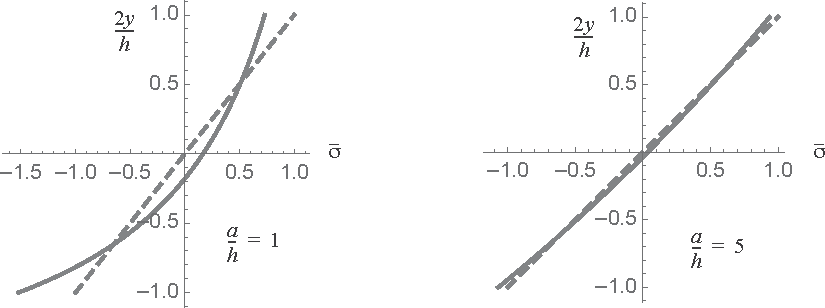
\includegraphics{Figure_7-4.pdf}
}{\caption{Thickness distributions of the dimensionless normal stress for $a/h = 1$ and $a/h = 5$. The solid line corresponds to the curved bar and the dashed line to the straight bar.\label{fig7.4}}\vspace*{10pt}}}




The error approximating the maximum stress from straight bar theory with respect to curved bar theory is 3.32 percent for $a / h=10$, and less than 1.66 percent for $a / h>20$.
\end{example}




\begin{example}[Displacement of a semicircular bar]\label{ex7.2}A semicircular bar of radius $a$ is connected to a fixed pin support at its left end and a pin support free to move horizontally at its right end. The right end support is subject to a horizontal force \textit{Q} with a corresponding displacement denoted by $q$. The cross section of the bar is the thin-walled tube of example~\ref{ex6.4} on page~\pageref{ex6.4} with the mean radius denoted by $b$, and a wall thickness denoted by $t$. See figure~\ref{fig7.5}. Determine the flexibility influence coefficient $c$ in the relation $q=c Q$ using Castigliano's second theorem.

{\def\thefigure{7.5}
\begin{figure}[!h]
\centering{\includegraphics{Figure_7-5.pdf}}
\caption{Configuration of the semicircular bar of example~\ref{ex7.2}, and its thin-walled cross section.\label{fig7.5}}
\end{figure}}

\subsubsection{Solution.}
The complementary strain energy in eq.~(\ref{eq7.26}) reduces to
\begin{equation}
U^{*}=\frac{1}{2 E a^{2} A} \int_{0}^{\pi}\left[(a N+M)^{2}+\frac{M^{2}}{Y}\right] a d \theta=\frac{1}{2 E a(2 \pi b t)} \int_{0}^{\pi}\left[(a N+M)^{2}+\frac{M^{2}}{Y}\right] d \theta. \label{eq7.2.a}\tag{a}
\end{equation}
A free body diagram of the segment of the bar is shown in figure~\ref{fig7.6}. The circumferential normal force \textit{N} and the bending moment \textit{M} determined from equilibrium are
{\def\thefigure{7.6}
\processfigure[H]{\includegraphics{Figure_7-6.pdf}
}{\caption{Free body diagram of a segment of the semicircular bar.\label{fig7.6}}}}
\vspace*{-2\baselineskip}
\begin{equation}
N=Q \sin \theta \quad M=-(a \sin \theta) Q. \label{eq7.2.b}\tag{b}
\end{equation}
From Castigliano's theorem the displacement corresponding to force \textit{Q} is given by
\begin{equation}
q=\frac{\partial U^{*}}{\partial Q}=\frac{1}{E a(2 \pi b t)} \int_{0}^{\pi}\left[(a N+M)\left(a \frac{\partial N}{\partial Q}+\frac{\partial M}{\partial Q}\right)+\frac{M}{Y} \frac{\partial M}{\partial Q}\right] d \theta. \label{eq7.2.c}\tag{c}
\end{equation}
Substitute for the actions \textit{N} and \textit{M} from eq. (\textbf{\ref{eq7.2.b}}) into eq. (\textbf{\ref{eq7.2.c}}) and perform the integral to get
\begin{equation}
q=\frac{Q}{E a(2 \pi b t)} \int_{0}^{\pi} \frac{a^{2} \sin ^{2} \theta}{Y} d \theta=\left(\frac{a}{4 E b t Y}\right) Q. \label{eq7.2.d}\tag{d}
\end{equation}
\vspace*{4pt}
\clearpage

\noindent Thus, the flexibility influence coefficient is identified in eq. (\textbf{\ref{eq7.2.d}}) as
\begin{equation}
c=\frac{a}{4 E b t Y}=\frac{\rho}{2 E t Y}, \label{eq7.2.e}\tag{e}
\end{equation}
in which the radius-to-thickness ratio is defined by $\rho=a /(2 b)$. The formula for the Winkler parameter \textit{Y} is obtained from the third expression in eq.~(\ref{eq7.19}) as
\begin{equation}
Y=\frac{1}{a A} \int \frac{y^{2}}{a+y} d A=\frac{1}{a(2 \pi b t)} \int_{0}^{2 \pi} \frac{(b \sin \varphi)^{2}}{a+b \sin \varphi} t b d \varphi=\frac{1}{4 \pi \rho} \int_{0}^{2 \pi} \frac{\sin ^{2} \varphi}{2 \rho+\sin \varphi} d \varphi. \label{eq7.2.f}\tag{f}
\end{equation}
The integration was performed in \textit{Mathematica} for $\rho>1 / 2$ to get
\begin{equation}
Y=\frac{2 \rho}{\sqrt{4 \rho^{2}-1}}-1. \label{eq7.2.g}\tag{g}
\end{equation}

Consider computing the flexibility influence coefficient from the complementary strain energy of a straight bar but applied to the semicircular bar. For this example eq.~(\ref{eq5.51}) on page~\pageref{eq5.51} reduces to the complementary energy expression
\begin{equation}
U^{*}=\frac{1}{\left(2 E I_{x x}\right)} \int_{0}^{\pi} M^{2} a d \theta+\frac{1}{2 E A} \int_{0}^{\pi} N^{2} a d \theta. \label{eq7.2.h}\tag{h}
\end{equation}

\vspace*{-1pc}

\noindent Let the displacement obtained from Castigliano's theorem using the complementary strain energy expression in eq. (\textbf{h}) be denoted by $q_{a}$. Then,
\begin{equation}
q_{a}=\left(\frac{1}{E I_{x x}}\right) \int_{0}^{\pi} M \frac{\partial M}{\partial Q} a d \theta+\frac{1}{E A} \int_{0}^{\pi} N \frac{\partial N}{\partial Q} a d \theta. \label{eq7.2.i}\tag{i}
\end{equation}
Substitute for the actions \textit{N} and \textit{M} from equilibrium eq. (\textbf{\ref{eq7.2.b}}) into eq. (\textbf{\ref{eq7.2.i}}) and perform the integral to get
\begin{equation}
q_{a}=\frac{a \pi Q}{2 A E}+\frac{a^{3} \pi Q}{2 I_{x x} E}=\frac{a Q}{4 b t E}+\frac{a^{3} Q}{2 b^{3} t E}, \label{eq7.2.j}\tag{j}
\end{equation}
in which we substitute for the area and second area moment $A=2\pi bt$ and $I_{x x}=\pi b^{3} t$, respectively. The approximate flexibility influence coefficient, denoted by $c_{a}$, is
\begin{equation}
c_{a}=\frac{a}{4 b t E}+\frac{a^{3}}{2 b^{3} t E}=\frac{\rho+8 \rho^{3}}{2 t E}, \label{eq7.2.k}\tag{k}
\end{equation}
where $\rho=a /(2 b)$.

The ratio of the flexibility influence coefficient in eq. (\textbf{\ref{eq7.2.e}}) to its approximate value in eq. (\textbf{\ref{eq7.2.k}}) is
\begin{equation}
c_{r}=c / c_{a}=\frac{1}{\left(1+8 \rho^{2}\right) Y}. \label{eq7.2.l}\tag{l}
\end{equation}
Numerical results for selected values of the radius-to-thickness ratios $\rho$ are presented in table~\ref{tab7.3}. The third column in the table lists the ratio of the flexibility influence coefficient to its approximate value. For $\rho= 1$ the approximate flexibility influence coefficient is about 1.39~$c$, which means the displacement $q_{a}$ is larger than the displacement determined from curved bar theory. For $\rho= 10 c_{a}=1.003~c$, and for $\rho$ exceeding ten, $c_{a}$ is essentially equal to $c$. Hence, we can use the strain energy expression for a straight bar to determine the displacement of the curved bar if $\rho \geq 10$.
\end{example}

\begin{table}%7.3
\processtable{Ratio of the exact flexibility coefficient to the
approximate value for selected radius-to-thickness ratios \label{tab7.3}}{
\tabcolsep=59pt\begin{tabular}{@{}lll@{}}
\toprule
\colhead{$\rho=a /(2 b)$} & \colhead{$Y(\rho)$} & \colhead{$c / c_{a}$} \\
\midrule
1 & 0.154701 & 0.718234 \\
2 & 0.0327956 & 0.923998 \\
3 & 0.0141851 & 0.965705\\
4 & 0.00790526 & 0.980605\\
5 & 0.00503782 & 0.987556\\
10 & 0.00125235 & 0.996879\\
\botrule
\end{tabular}}{}
\vspace*{-6pt}
\end{table}

\section{Strain-displacement and Hooke's law for thin curved bars}\label{sec7.2}

It was demonstrated in example~\ref{ex7.1} and example~\ref{ex7.2} that some equations of straight bar theory are applicable to the analysis of curved bars if the radius of curvature to the thickness in the plane of curvature is greater than ten. If the ratio of the minimum radius of curvature to the in-plane thickness is greater than ten, then the bar is identified as a \textbf{thin curved bar}. Ratios less than ten are considered \textbf{thick curved bars}. For example, thin curved bar formulas are applicable to fuselage ring-frames. Fittings, machine parts, crane hooks, and chain links are examples where thick curved bar theory is required. Thin curved bar formulas for strain, stress, stress resultants, and complementary strain energy are as follows:\vspace*{-6pt}
\begin{gather}
\varepsilon=\frac{d w}{d s}+\frac{v}{R}-y\left(\frac{d^{2} v}{d s^{2}}+\frac{w}{R^{2}} \frac{d R}{d s}\right), \label{eq7.27} \\
N=E A\left(\frac{d w}{d s}+\frac{v}{R}\right) \quad M=-E I_{x x}\left(\frac{d^{2} v}{d s^{2}}+\frac{w}{R^{2}} \frac{d R}{d s}\right), \textrm{ and} \label{eq7.28} \\
\sigma=E \varepsilon=\frac{N}{A}+y \frac{M}{I_{x x}} \quad U^{*}=\frac{1}{2} \int\left(\frac{N^{2}}{E A}+\frac{M^{2}}{E I_{x x}}\right) d s. \label{eq7.29}
\end{gather}

\vspace*{-6pt}
\begin{example}[Circular arch]\label{ex7.3}Consider a thin curved bar that forms a circular arch as shown in figure~\ref{fig7.7}. It is supported by smooth pins at each end. The distance \textit{L} between the end supports remains fixed as the arch is subject to a downward force \textit{P} at midspan. The area of the cross section is denoted by \textit{A}, the radius of the circular arc passing through the centroid of each cross section by $a$, and its semi-opening angle by $\beta$. The arch is statically indeterminate and the horizontal reaction force \textit{Q} is the redundant. The overall free body diagram of the arch is shown in figure~\ref{fig7.7}.
\begin{enumerate}[(a)]\leftskip3pt
\item[(a)] Using Castigliano's second theorem determine the redundant load \textit{Q}. Neglect strain energy due to transverse shear.

\item[(b)] Take $L = 1$~m, $E A=175\times 10^{6}\,\mathrm{N}$, and $E I=218,750\,\mathrm{N}$-$\mathrm{m}^{2}$. Plot \textit{Q/P} as function of the rise to span ratio \textit{H/L} for $1^{\circ} \leq \beta \leq 90^{\circ}$.
\end{enumerate}


{\def\thefigure{7.7}
\processfigure{\includegraphics{Figure_7-7.pdf}
}{\caption{Circular arch. $a/h > \textbf{10}$.\label{fig7.7}}}}


\subsubsection{Solution to part (a).} The arch is symmetric about the vertical axis through the center, so only the left-half section is analyzed. The free body diagram shown in figure~\ref{fig7.8} cuts the arch at angle $\theta$ measured counterclockwise from the vertical axis, and $0 \leq \theta \leq \beta$. The internal actions on the cut face are the circumferential normal force \textit{N}, transverse shear force \textit{V}, and the bending moment \textit{M}. The cut face is a negative $\theta$-face with a positive normal force causing circumferential extension, a positive shear force is defined radially inward, and a positive bending moment causes tension on the radially outboard circumference.

\begin{wrapfigure}[17]{R}{210.9pt}
\vspace{-30pt}
\includegraphics{Figure_7-8.pdf}
\caption{Free body diagram of a section of the arch\vspace*{16pt}.\label{fig7.8}}
\end{wrapfigure}

Equilibrium in the direction of the normal force leads to the equation
\begin{equation}
N=-(P / 2) \sin \theta-Q \cos \theta. \label{eq7.3.a}\tag{a}
\end{equation}
Equilibrium in the direction of the shear force leads to the equation
\begin{equation}
V=(P / 2) \cos \theta-Q \sin \theta. \label{eq7.3.b}\tag{b}
\end{equation}
Moment equilibrium at the $\theta$-face leads to the equation
\begin{equation}
M=-a(\sin \beta-\sin \theta)(P / 2)+a(\cos \theta-\cos \beta) Q. \label{eq7.3.c}\tag{c}
\end{equation}
The complementary strain energy from eq.~(\ref{eq7.29}) redu\-ces~\vspace*{10pt}to
\begin{equation}
U^{*}=2\left(\frac{1}{2}\right) \int_{0}^{\beta}\left[\frac{N^{2}}{2 E A}+\frac{M^{2}}{2 E I}\right] a d \theta. \label{eq7.3.d}\tag{d}
\end{equation}
In the previous integral, integration is performed over the left-hand portion of the arch, and the total complementary energy stored in the arch is accounted for by the factor of two multiplying the integral. Since the displacement in the direction of the horizontal redundant force \textit{Q} is zero, Castigliano's second theorem gives $0=\left(\partial U^{*}\right) /(\partial Q)$. Thus,
\begin{equation}
0=\int_{0}^{\mathrm{\beta}}\left[\frac{N}{E A}\left(\frac{\partial N}{\partial Q}\right)+\frac{M}{E I}\left(\frac{\partial M}{\partial Q}\right)\right] a d \theta. \label{eq7.3.e}\tag{e}
\end{equation}
Substitute eq. (\textbf{\ref{eq7.3.a}}) for \textit{N} and eq. (\textbf{\ref{eq7.3.c}}) for \textit{M} in eq. (\textbf{\ref{eq7.3.e}}) followed by integration to get
\begin{align}
0=\left(\frac{a}{2 E A}\right) &\left[\sin ^{2} \beta P+(2 \beta+\sin 2 \beta) Q\right]+ \nonumber\\
&\left(\frac{a^{3}}{4 E I}\right)[(1-4 \cos \beta+3 \cos 2 \beta+2 \beta \sin 2 \beta) P+(8 \beta+4 \beta \cos 2 \beta-6 \sin 2 \beta) Q]. \label{eq7.3.f}\tag{f}
\end{align}
Solve eq. (\textbf{\ref{eq7.3.f}}) for the redundant force \textit{Q} to get
\begin{equation}
\frac{Q}{P}=\frac{a^{2}(-1+4 \cos \beta-3 \cos 2 \beta-2 \beta \sin 2 \beta) E A-\left(2 \sin ^{2} \beta\right) E I}{a^{2}(8 \beta+4 \beta \cos 2 \beta-6 \sin 2 \beta) E A+(4 \beta+2 \sin 2 \beta) E I}. \label{eq7.3.g}\tag{g}
\end{equation}

\subsubsection{Solution to part (b).} The rise-to-span ratio in terms of the semi-opening angle $\beta$ is
\begin{equation}
\frac{H}{L}=\frac{a(1-\cos \beta)}{2 a \sin \beta}=\frac{(1-\cos \beta)}{2 \sin \beta}. \label{eq7.3.h}\tag{h}
\end{equation}
Note that this ratio is independent of the radius $a$. The distance \textit{L} between the supports is fixed at one meter, and $L=2 a \sin \beta$. Hence, the radius of the arch is a function of the semi-opening angle $\beta$ given by
\begin{equation}
a=(1\,\mathrm{m}) /(2 \sin \beta). \label{eq7.3.i}\tag{i}
\end{equation}
Specifying $\beta$, we compute $a$ from eq. (\textbf{i}), \textit{H/L} from eq. (\textbf{\ref{eq7.3.h}}), and the ratio of \textit{Q/P} from eq. (\textbf{\ref{eq7.3.g}}). A graph of \textit{Q/P} versus \textit{H/L} is shown in figure~\ref{fig7.9}.

{\def\thefigure{7.9}
\processfigure[H]{\includegraphics{Figure_7-9.pdf}
}{\caption{Ratio of the horizontal reaction force to the applied load as a function of the rise-to-span ratio for a circular arch.\label{fig7.9}}}}
\vspace*{-\baselineskip}


\noindent The maximum value of the redundant is \textit{2P} for $\textit{H/L} = 0.0485$ corresponding to $\beta=11.08^{\circ}$. This maximum occurs for a shallow arch. A shallow arch is characterized by a small value of the angle $\beta$.
\end{example}

\vspace*{-6pt}
\begin{example}[Thin ring subject to diametric tension]\label{ex7.4}A uniform, thin ring of radius $a$ is subject to equal and opposite tension forces labeled \textit{P} as shown in the left sketch in figure~\ref{fig7.10}. This configuration is symmetric about the horizontal diameter AB and the vertical diameter. Determine the bending moment distribution in the upper right-hand quarter segment of the ring where the angle $\theta$ has the range $0 \leq \theta \leq \pi / 2$. Include only bending deformations in Castigliano's second theorem to determine the redundant actions.

\subsubsection{Solution.} The right-hand sketch in figure~\ref{fig7.10} shows the free body diagrams obtained by sectioning the ring across diameter AB. Action-reaction pairs of the internal circumferential normal forces, internal transverse shear forces, and internal bending moments are labeled in the free body diagrams. The upper and lower free body diagrams are mirror images of one another, which implies that the transverse shear forces $V_{A}$ in the upper and lower free body diagrams should be drawn in the same direction at the cut at \textit{A}. But this mirror image argument is in contradiction with the action-reaction pairing. So to resolve this contradiction means that the transverse shear force $V_{A}=0$. A similar argument implies that the transverse shear force at cut \textit{B} must vanish (i.e., $V_{B}=0$).

{\def\thefigure{7.10}
\begin{figure}[!h]
\centerline{\includegraphics{Figure_7-10.pdf}}
\caption{A thin ring subject to diametric tension. Free body diagrams obtained from a cut across the horizontal diameter.}\label{fig7.10}
\vspace*{4pt}
\end{figure}}
%\vspace*{-\baselineskip}

From symmetry about the vertical diameter the circumferential normal forces $N_{A}$ and $N_{B}$ are equal and the bending moments $M_{A}$ and $M_{B}$ are equal. Vertical force equilibrium yields $N_{A}=N_{B}=P / 2$. Thus, the only redundant is the bending moment $M_{A}$. A free body diagram of the section from point A to the cut at $\theta$ is shown in figure~\ref{fig7.11}.


{\def\thefigure{7.11}
\vspace*{-\baselineskip}
\processfigure[H]{\includegraphics{Figure_7-11.pdf}
}{\caption{Free body diagram of a circular sector of the ring in example~\ref{ex7.4}.\label{fig7.11}}\vspace*{-10pt}}}
\vspace*{-\baselineskip}

Moment equilibrium about the cut at $\theta$ determines the bending moment as
\begin{equation}
M=M_{A}+a(1-\cos \theta)(P / 2). \label{eq7.4.a}\tag{a}
\end{equation}

\noindent The complementary strain energy including bending only is
\begin{equation}
U^{*}=\int_{0}^{\frac{\pi}{2}}\left[\frac{M^{2}}{2 E I}\right] a d \theta. \label{eq7.4.b}\tag{b}
\end{equation}
By symmetry, the rotation corresponding to the moment $M_{A}$ must vanish. Hence, Castigliano's second theorem gives
\begin{equation}
0=\frac{\partial U^{*}}{\partial M_{A}}=\frac{1}{E I} \int_{0}^{\frac{\pi}{2}}[M]\left[\frac{\partial M}{\partial M_{A}}\right] a d \theta=\frac{1}{E I} \int_{0}^{\frac{\pi}{2}}\left[M_{A}+a(1-\cos \theta)(P / 2)\right][1] a d \theta. \label{eq7.4.c}\tag{c}
\end{equation}
Perform the integration in eq. (\textbf{\ref{eq7.4.c}}) to get
\begin{equation}
0=\frac{1}{E I}\left[\frac{M_{A} \pi a}{2}-\frac{P a^{2}}{2}+\frac{1}{4} P \pi a^{2}\right]. \label{eq7.4.d}\tag{d}
\end{equation}
Solve eq. (\textbf{\ref{eq7.4.d}}) for the redundant to find
\begin{equation}
M_{A}=\frac{P a(2-\pi)}{2 \pi}. \label{eq7.4.e}\tag{e}
\end{equation}
Substitute eq. (\textbf{\ref{eq7.4.e}}) into eq. (\textbf{\ref{eq7.4.a}}) to get the bending moment as
\begin{equation}
M=\frac{P a}{\pi}-\frac{1}{2} P a \cos \theta \quad 0 \leq \theta \leq \frac{\pi}{2}. \label{eq7.4.f}\tag{f}
\end{equation}
The bending moment is plotted in figure~\ref{fig7.12} as a radial coordinate with respect to the ring, where a positive moment is plotted outside the ring and a negative moment is plotted inside the ring.
\end{example}

{\def\thefigure{7.12}
\processfigure[H]{\includegraphics{Figure_7-12.pdf}
}{\caption{Bending moment distribution in one quarter of the ring, which is subject to diametric tension.\label{fig7.12}}}}

\pagebreak

\section{Differential equilibrium equations of a curved bar}\label{sec7.3}

Consider a differential element of a curved bar subject to prescribed line load per unit length along the reference axis. The vector of the external line load intensity is denoted by $\harp{f}(s)$ with component $q(s)$ tangent to the reference axis and component $p(s)$ normal to the reference axis. That is
\begin{align}\label{eq7.30}
\harp{f}(s)=q(s) \hat{t}(s)+p(s) \hat{j}(s).
\end{align}
Denote the internal force vector acting on the cross section by $\harp{F}(s)$ with component $N(s)$ normal to the cross section positive in tension, and the shear component $V(s)$ tangent to the cross section. That is,
\begin{align}\label{eq7.31}
\harp{F}(s)=N(s) \hat{t}(s)+V(s) \hat{j}(s).
\end{align}
Summation of forces acting on the differential element shown in figure~\ref{fig7.13} leads to
{\def\thefigure{7.13}
\processfigure[H]{\includegraphics{Figure_7-13.pdf}
}{\caption{Free body diagram of an element of a curved bar.\label{fig7.13}}}}
\vspace*{-2\baselineskip}

\begin{align}\label{eq7.32}
\harp{F}(s+d s)-\harp{F}(s)+\harp{f}\left(s^{*}\right) d s=0 \quad s<s^{*}<s+d s.
\end{align}
Expanding the force vectors in a series we write eq.~(\ref{eq7.32}) as
\begin{align}\label{eq7.33}
\left\{\frac{d \harp{F}}{d s}+\left[\harp{f}(s)+\frac{d \dot{f}}{d s}\left(s^{*}-s\right)\right]\right\} d s+O(d s^{2})=0.
\end{align}
Divide eq.~(\ref{eq7.33}) by \textit{ds}, followed by taking the limit as $d s \rightarrow 0$, and note that $s^{*} \rightarrow s$ in the limit. The resulting differential equation is
\begin{align}\label{eq7.34}
\frac{d \harp{F}}{d s}+\harp{f}(s)=0.
\end{align}
The derivative of the internal force vector in eq.~(\ref{eq7.31}) is
\begin{equation*}
\frac{d \harp{F}}{d s}=\left(\frac{d N}{d s}\right) \hat{t}+N\left(\frac{d \hat{t}}{d s}\right)+\left(\frac{d V}{d s}\right) \hat{j}+V\left(\frac{d \hat{j}}{d s}\right)=\left(\frac{d N}{d s}+\frac{V}{R}\right) \hat{t}+\left(\frac{d V}{d s}-\frac{N}{R}\right) \hat{j},
\end{equation*}
where the derivatives of the unit vectors are given in eq.~(\ref{eq7.3}). Hence, the scalar differential equation of force equilibrium in the tangent direction is
\begin{align}\label{eq7.35}
\frac{d N}{d s}+\frac{V}{R}+q=0,
\end{align}
and differential equation in the normal direction is
\begin{align}\label{eq7.36}
\frac{d V}{d s}-\frac{N}{R}+p=0.
\end{align}

The bending moment acting on the cross section is denoted by $M(s)$ with a positive moment causing an increase in curvature of the bar. Take the sum of moments about $s$ in the free body diagram to get
\begin{align}\label{eq7.37}
M(s+d s) \hat{i}-M(s) \hat{i}+[\harp{r}(s+d s)-\harp{r}(s)] \times \harp{F}(s+d s)+\left[\harp{r}\left(s^{*}\right)-\harp{r}(s)\right] \times \harp{f}\left(s^{*}\right) d s=0,
\end{align}
Expanding the moment and force vector in a series we write
\begin{align}\label{eq7.38}
\left\{\frac{d M}{d s} \hat{i}+\frac{d \dot{r}}{d s} \times \harp{F}(s)+\left[\hat{r}\left(s^{*}\right)-\hat{r}(s)\right] \times \bar{f}\left(s^{*}\right)\right\} d s+O(d s^{2})=0.
\end{align}
Divide by \textit{ds} and then take the limit as $d s \rightarrow 0$, and note that $\harp{r}\left(s^{*}\right) \rightarrow \harp{r}(s)$ in the limit, to get
\begin{align}\label{eq7.39}
\frac{d M}{d s} \hat{i}+\hat{t} \times[N \hat{t}+\hat{j j}]=\left(\frac{d M}{d s}-V\right) \hat{i}=0.
\end{align}
The moment differential equation is
\begin{align}\label{eq7.40}
\frac{d M}{d s}-V=0.
\end{align}

\begin{example}[Funicular arch]\label{ex7.5}Consider a uniform, pinned-pinned arch subject to uniformly distributed load of intensity $p_0$ that is directed vertically downward as shown in figure~\ref{fig7.14}. For example $p_0$ could represent the weight per unit length of the arch. We determine the form or shape of the arch such that each cross section is in pure compression (i.e., there is no bending). This condition of pure compression under a uniform lateral load can be achieved with a curved bar, but not with a straight bar or beam. A beam carries a uniform lateral load by bending. Tailoring the shape of the arch for pure compression to the uniformly distributed loading defines the funicular arch. All of the parallel fibers in a cross section are under the same compressive stress, which means all of the material in the cross section is utilized in resisting the load.

{\def\thefigure{7.14}
\processfigure{\includegraphics{Figure_7-14.pdf}
}{\caption{Funicular arch subject to a uniformly distributed load.\label{fig7.14}}}}


Resolve the applied downward load intensity into the tangential and normal components of eq.~(\ref{eq7.30}) to find
\begin{equation}
q=p_{0} \sin \theta \quad p=-p_{0} \cos \theta. \label{eq7.5.a}\tag{a}
\end{equation}
For the bending moment and shear force to vanish for all values of $s$ the equilibrium equations (\ref{eq7.35}) to (\ref{eq7.40}) reduce to the following:
\begin{equation}
\frac{1}{R} \frac{d N}{d \theta}+p_{0} \sin \theta=0 \quad-\frac{N}{R}-p_{0} \cos \theta=0. \label{eq7.5.b}\tag{b}
\end{equation}
\vadjust{\pagebreak}

\noindent Eliminating the tangential force between the last two equations leads to the following differential equation for the radius of curvature:
\begin{equation}
\frac{d R}{d \theta}-(2 \tan \theta) R=0. \label{eq7.5.c}\tag{c}
\end{equation}
The solution for the radius of curvature is
\begin{equation}
R=\frac{a}{\cos ^{2} \theta}, \label{eq7.5.d}\tag{d}
\end{equation}
where $a$ is the constant of integration and is equal to the radius of curvature at $\theta= 0$. The curvature is $1/R$ and from the third expression in eq.~(\ref{eq7.3}) we obtain
\begin{equation}
\frac{d \theta}{d s}=\frac{\cos ^{2} \theta}{a} \rightarrow \int \sec ^{2} \theta d \theta=\int \frac{1}{a} d s. \label{eq7.5.e}\tag{e}
\end{equation}

\begin{wrapfigure}[6]{r}{64pt}
%\vspace{-19pt}
\includegraphics{Figure_7-15.pdf}
\caption{\label{fig7.15}}
\end{wrapfigure}

\vspace*{-0.5pc}

\noindent Perform the integration in eq. (\textbf{\ref{eq7.5.e}}) to find $\tan \theta=s/a$. From the result that the tangent of $\theta$ is equal to the arc-length divided by $a$, we obtain the trigonometric relations (see figure~\ref{fig7.15})
\begin{equation}
\sin \theta=\frac{s}{\sqrt{a^{2}+s^{2}}} \quad \text { and } \quad \cos \theta=\frac{a}{\sqrt{a^{2}+s^{2}}}. \label{eq7.5.f}\tag{f}
\end{equation}
As shown by the insert in figure~\ref{fig7.1}, $\left(d z_{0}\right) /(d s)=\cos \theta$, which combined with the cosine relation from eq. (\textbf{\ref{eq7.5.b}}) can be integrated to determine coordinate function $z_{0}(s)$; i.e.,
\begin{equation*}
z_{0}=\int \frac{a}{\sqrt{a^{2}+s^{2}}} d s=\int \frac{a}{\sqrt{1+\left(\frac{s}{a}\right)^{2}}} d\left(\frac{s}{a}\right)=a \sinh ^{-1} \frac{s}{a}.
\end{equation*}
Thus,
\begin{equation}
\sinh \left(z_{0} / a\right)=s / a. \label{eq7.5.g}\tag{g}
\end{equation}
Also as shown by the insert in figure~\ref{fig7.1}, $\left(d y_{0}\right) /(d s)=-\sin \theta$, which combined with the sine relation from eq. (\textbf{\ref{eq7.5.f}}) can be integrated to determine coordinate function $y_{0}(s)$; i.e.,
\begin{equation}
y_{0}=\int \frac{-s}{\sqrt{a^{2}+s^{2}}} d s=-\sqrt{a^{2}+s^{2}}+c. \label{eq7.5.h}\tag{h}
\end{equation}
We specify $y_{0}(0)=a$, and find $c=2 a$. The coordinate function $y_{0}(s)$ is
\begin{equation}
y_{0}=2 a-\sqrt{a^{2}+s^{2}}. \label{eq7.5.i}\tag{i}
\end{equation}
Express eq. (\textbf{\ref{eq7.5.i}}) as $y_{0}=2 a-a \sqrt{1+(s / a)^{2}}$, and use eq. (\textbf{\ref{eq7.5.g}}) to replace the ratio \textit{s/a} to get
\begin{equation}
y_{0}=2 a-a \sqrt{1+\sinh ^{2} \frac{z_{0}}{a}}=2 a-a \sqrt{\cosh ^{2} \frac{z_{0}}{a}}. \label{eq7.5.j}\tag{j}
\end{equation}
The latter result in eq. (\textbf{\ref{eq7.5.j}}) is the equation for the shape of the funicular arch, which is
\begin{equation}
y_{0}=2 a-a \cosh \left(z_{0} / a\right). \label{eq7.5.k}\tag{k}
\end{equation}
Equation (\textbf{\ref{eq7.5.k}}) is the equation of a \textbf{catenary}. A catenary is a curve formed by a wire, rope, or chain hanging freely from two points that is in tension. The funicular arch is an inverted catenary and is in compression.



The tangential force in the arch is given by $N=-p_{0} R \cos \theta$. Using eqs. (\textbf{\ref{eq7.5.d}}), (\textbf{\ref{eq7.5.f}}), and (\textbf{\ref{eq7.5.g}}), it can be shown that the spanwise distribution of the tangential force is
\begin{equation}
N=-p_{0} a \cosh \left(z_{0} / a\right), \label{eq7.5.l}\tag{l}
\end{equation}
where $-z_{m} / a \leq z_{0} / a \leq z_{m} / a$. Set $y_{0}=0$ in eq. (\textbf{\ref{eq7.5.k}}) to find $z_{m} / a=\operatorname{ArcCosh}\;(2)=1.317$. Define the thrust as the negative of the tangential force. The spanwise distribution of the thrust scaled by $p_{0} a$ is shown in figure~\ref{fig7.16}. The minimum thrust is $p_{0} a$ at the crown and increases to a maximum of $2 p_{0} a$ at each pin support.
\end{example}

{\def\thefigure{7.16}
\vspace*{-\baselineskip}
\processfigure[H]{\includegraphics{Figure_7-16.pdf}
}{\caption{Distribution of the thrust with respect to the span of the funicular arch, $\textit{z}_{\textrm{m}}/a = \textbf{1.317}$.\label{fig7.16}}}}
\vspace*{-1.6\baselineskip}


\section{Loads on fuselage frames}\label{sec7.4}

The skins, or webs, in semimonocoque construction are thin and cannot withstand large concentrated loads. Instead, stiffeners are located into the design of the structure where the concentrated loads are applied. The concentrated load acting on the stiffener diffuses the load to the attached skins or webs. For example, a fuselage structure has closely spaced frames or bulkheads that resist loads in the transverse planes, while the fuselage shell resist loads in the fore-and-aft direction. Typically, frames react to point loads from the wing spar attachments and distributed loads from floor beams, and are often modeled as two-dimensional rings subject to in-plane loading. In the following analyses, we quantitatively determine how loads applied to frames are transferred to the\vadjust{\vspace*{10pt}\pagebreak} attached skin, followed by the determination of the internal actions in the frame. Additional examples of loads acting on fuselage frames and wing ribs are given in Bruhn (1973), Curtis (1997), and Megson (1999).

{\def\thefigure{7.17}
\processfigure[H]{\includegraphics{Figure_7-17.pdf}
}{\caption{(a) Frame loads. (b) Forces and torques acting on frame and fuselage skin viewed from the\break $y$-$z$ plane. (c) Shear flows in the skin fore and aft of the frame and the interface shear flow from the frame acting on the skin.\label{fig7.17}}}}


Consider a transverse frame together with the attached skin of the fuselage. The frame is subject to forces $P_{x}$ and $P_{y}$, and torque $T_{z}$ as shown in figure~\ref{fig7.17}(a). Note that positive values of $P_{x}$ and $P_{y}$ are defined in the negative $x$- and $y$-directions, respectively, and a positive torque is defined in the negative $z$-direction by the right-hand screw rule. Equilibrium immediately fore and aft of the frame leads to jumps in the shear forces and torque acting on the fuselage skin. As depicted in figure~\ref{fig7.17}(b), the jump conditions are
\begin{align}\label{eq7.41}
\Delta V_{x}=V_{x}^{+}-V_{x}^{-}=P_{x} \quad \Delta V_{y}=V_{y}^{+}-V_{y}^{-}=P_{y} \quad \Delta M_{z}=M_{z}^{+}-M_{z}^{-}=T_{z}.
\end{align}
As shown in figure~\ref{fig7.17}(c) the shear flows acting on the cross section of the fuselage immediately fore and aft of the frame are denoted by $q^{+}$ and $q^{-}$, respectively. The shear flow exerted by the frame on the skin at the interface is denoted by $\bar{q}$. Equilibrium of the shear flows in figure~\ref{fig7.17}(c) yields
\begin{align}\label{eq7.42}
q^{+}-q^{-}=\bar{q}.
\end{align}
The shear flow acting on a single-cell cross section is given by eq.~(\ref{eq3.163}) on page \pageref{eq3.163}. For this situation
\begin{align}\label{eq7.43}
q(s, z)=\frac{M_{z}}{2 A_{c}}-F_{x}(s) V_{x}(z)-F_{y}(s) V_{y}(z).
\end{align}

\vspace*{-1pc}

Assume the geometry of the fuselage shell is the same fore and aft of the frame. Substitute eq.~(\ref{eq7.43}) for the shear flows in the skin fore and aft of the frame into eq.~(\ref{eq7.42}) to find the shear flow exerted on the skin by the frame as
\begin{align}\label{eq7.44}
\bar{q}=-F_{x}(s)\left[V_{x}^{+}-V_{x}^{-}\right]-F_{y}(s)\left[V_{y}^{+}-V_{y}^{-}\right]+\left[M_{z}^{+}-M_{z}^{-}\right] /\left(2 A_{c}\right).
\end{align}
Now substitute the jump conditions from eq.~(\ref{eq7.41}) into eq.~(\ref{eq7.44}) to get
\begin{align}\label{eq7.45}
\bar{q}=-F_{x}(s) P_{x}-F_{y}(s) P_{y}+T_{z} /\left(2 A_{c}\right).
\end{align}
Since the shear center and centroid coincide, the shear flow distribution functions from eqs. (\ref{eq3.151}) and (\ref{eq3.164}) on page~\pageref{eq3.151} and page~\pageref{eq3.164}, respectively, are given by
\begin{align}\label{eq7.46}
F_{x}(s)=\frac{1}{I_{y y}}\left[Q_{y}(s)-\frac{1}{2 A_{c}} \oint\left(r_{n} Q_{y}\right) d s\right] \quad F_{y}(s)=\frac{1}{I_{x x}}\left[Q_{x}(s)-\frac{1}{2 A_{c}} \oint\left(r_{n} Q_{x}\right) d s\right].
\end{align}
Equation (\ref{eq7.45}) determines the interface shear flow exerted by the frame on the fuselage skin in terms of the concentrated loads acting on the frame as depicted in figure~\ref{fig7.18}(a). The reaction to this interface shear flow acts on the frame, and the free body diagram of the frame is shown in figure~\ref{fig7.18}(b).

{\def\thefigure{7.18}
\processfigure[H]{\includegraphics{Figure_7-18.pdf}
}{\caption{(a) Free body diagram\break of the fuselage skin. (b) Free body diagram of the frame.\label{fig7.18}}}}

\vspace*{-2\baselineskip}

\begin{example}[Floor loading on a frame in a stringer-stiffened fuselage]\label{ex7.6}
\begin{wrapfigure}[18]{L}{183pt}
\vspace{-30pt}
\includegraphics{Figure_7-19.pdf}
\caption{Fuselage frame.\label{fig7.19}}
\end{wrapfigure}
\vspace*{-2\baselineskip}

A frame in a circular fuselage is subject to a uniformly distributed line load with an intensity of 12 lb./in. acting on its floor support. See the adjacent sketch. The fuselage skin thickness $t=0.015 \textrm{ in}$., and it is stiffened by six stringers spaced $60^{\circ}$ apart. Stringers 1, 2, 4, and 5 have flange areas $A_{f}=0.15 \textrm{ in.}^{2}$, and stringers 3 and 6 have flange areas $2 A_{f}=0.30 \textrm{ in.}^{2}$. Determine the interface shear flows acting on the skin-stringer fuselage due to the contact with the frame.

\subsubsection{Solution.} The circular skin-stringer fuselage is symmetric with respect to the $x$- and $y$-axes through its center, so the centroid and shear center are both located at the center of the circle. The resultant downward force acting on the frame is $P_{y}=12 \times 86.6=1,039.2 \textrm{ lb}$. When the frame is removed from the fuselage the action of the frame on the fuselage is represented by a jump in the shear force in the fuselage. From eq.~(\ref{eq7.41}) $\Delta V_{y}=P_{y}$. A free body diagram of the skin-stringer structure is shown in figure~\ref{fig7.20}.

{\def\thefigure{7.20}
\processfigure{\includegraphics{Figure_7-20.pdf}
}{\caption{Free body diagram of the skin-stringer\break structure. \phantom{000}\label{fig7.20}}}}




The expression (\ref{eq7.45}) for the interface shear flow in this example reduces to $\bar{q}=-F_{y}(s) P_{y}$. The contour coordinate $s$ is related to the polar angle $\theta$ by $s=a \theta$, where the radius of the circular contour $a=50 \text { in. }$, and $0 \leq \theta<2 \pi$ radians. The contour distribution function $F_{y}(s)$, or $F_{y}(\theta)$, is given by eq.~(\ref{eq7.46}), which is a evaluated by computing the first area moment with respect to the $x$-axis of a portion of the skin-stringer fuselage from $\theta=-\pi / 2$ to a value in the range $-\pi / 2<\theta<3 \pi / 2$. The expression for the first area moment $Q_{x}(\theta)$ is facilitated by accumulating the first area moments in each of the six segments of the contour\vadjust{\vspace*{6pt}\pagebreak}.

Beginning at $\theta=-\pi / 2$, and proceeding counterclockwise around the contour, the first area moments of the skin-stringer structure with respect to the $x$-axis are denoted by $Q_{x i}(\theta)$, $i=1,2, \ldots, 6$. The first area moments are calculated as follows:
\begin{gather}
Q_{x 1}(\theta)=-a\left(2 A_{f}\right)+\int_{-\pi / 2}^{\theta}(a \sin \theta) t a d \theta=-a\left(2 A_{f}\right)-a^{2} t \cos \theta \quad-\pi / 2 \leq \theta<-\pi / 6, \label{eq7.6.a}\tag{a} \\
Q_{x 2}(\theta)=Q_{x 1}\left(-\frac{\pi}{6}\right)+\left(-\frac{a}{2}\right) A_{f}+\int_{-\pi / 6}^{\theta}(a \sin \theta) \operatorname{tad} \theta=-\frac{a}{2}\left(5 A_{f}+2 a t \cos \theta\right) \quad-\pi / 6 \leq \theta<\pi / 6, \label{eq7.6.b}\tag{b} \\
Q_{x 3}(\theta)=Q_{x 2}\left(\frac{\pi}{6}\right)+\left(\frac{a}{2}\right) A_{f}+\int_{\pi / 6}^{\theta}(a \sin \theta) \operatorname{ta} d \theta=-a\left(2 A_{f}+a t \cos \theta\right) \quad \pi / 6 \leq \theta<\pi / 2, \label{eq7.6.c}\tag{c} \\
Q_{x 4}(\theta)=Q_{x 3}\left(\frac{\pi}{2}\right)+a\left(2 A_{f}\right)+\int_{\pi / 2}^{\theta}(a \sin \theta) \operatorname{tad} \theta=-a^{2} t \cos \theta \quad \pi / 2 \leq \theta<5 \pi / 6, \label{eq7.6.d}\tag{d} \\
Q_{x 5}(\theta)=Q_{x 4}\left(\frac{5 \pi}{6}\right)+\left(\frac{a}{2}\right) A_{f}+\int_{5 \pi / 6}^{\theta}(a \sin \theta) \operatorname{tad} \theta=\frac{a}{2}\left(A_{f}-2 a t \cos \theta\right) \quad 5 \pi / 6 \leq \theta<7 \pi / 6, \textrm{ and}\label{eq7.6.e}\tag{e}\\
Q_{x 6}(\theta)=Q_{x 5}\left(\frac{7 \pi}{6}\right)+\left(-\frac{a}{2}\right) A_{f}+\int_{7 \pi / 6}^{\theta}(a \sin \theta) \operatorname{ta} d \theta=-a^{2} t \cos \theta \quad 7 \pi / 6 \leq \theta<3 \pi / 2. \label{eq7.6.f}\tag{f}
\end{gather}
Note that the first area moment of the entire cross section about the $x$-axis vanishes, or $Q_{x 6}(3 \pi / 2)=0$, since the $x$-axis passes through the centroid.

The expression for the shear flow distribution function from eq.~(\ref{eq7.46}) is written as
\begin{equation}
F_{y i}(\theta)=\frac{1}{I_{x x}}\left[Q_{x i}(\theta)-\frac{1}{2 A_{c}} \oint\left(r_{n} Q_{x}\right) a d \theta\right] \quad i=1,2 \ldots, 6. \label{eq7.6.g}\tag{g}
\end{equation}
The integral of $r_{n} Q_{x}$ around the entire contour, where $r_{n}=a$, is given by
\begin{equation}
\begin{gathered}\oint\left(r_{n} Q_{x}\right) a d \theta=\int_{-\pi / 2}^{-\pi / 6} a Q_{x 1}(\theta) a d \theta+\int_{-\pi / 6}^{\pi / 6} a Q_{x 2}(\theta) a d \theta+\int_{\pi / 6}^{\pi / 2} a Q_{x 3}(\theta) a d \theta+\int_{\pi / 2}^{5\pi / 6} a Q_{x 4}(\theta) a d \theta \\
+ \int_{5 \pi / 6}^{7 \pi / 6} a Q_{x 5} (\theta) a d \theta+\int_{7 \pi / 6}^{3\pi / 2} a Q_{x 6}(\theta) a d \theta\end{gathered}, \label{eq7.6.h}\tag{h}
\end{equation}
which after integration yields
\begin{equation}
\oint\left(r_{n} Q_{x}\right) a d \theta=-2 \pi a^{3} A_{f}. \label{eq7.6.i}\tag{i}
\end{equation}
The area enclosed by the contour is $A_{c}=a^{2} \pi$. Hence, the interface shear flows are given by
\begin{equation}
\bar{q}_{i}(\theta)=-\left(\frac{1}{I_{x x}}\right)\left[Q_{x i}(\theta)+a A_{f}\right] P_{y} \quad i=1,2 \ldots, 6. \label{eq7.6.j}\tag{j}
\end{equation}
The second area moment about the $x$-axis is given by
\begin{equation}
I_{x x}=\int_{0}^{2 \pi}(a \sin \theta)^{2} t a d \theta+\sum_{i=1}^{6}\left(y f_{i}\right)^{2} A f_{i}=5 a^{2} A_{f}+\pi a^{3} t=7,765.49 \textrm{ in.}^{4}\label{eq7.6.k}\tag{k}
\end{equation}
Results for the interface shear flows with dimensional units of lb./in. are listed below:
\begin{gather}
\bar{q}_{1}(\theta)=\left[\frac{a(A_{f}+a t \cos \theta)}{I_{x x}}\right] P_{y}=1.00367+5.01836 \cos \theta \quad-\pi / 2 \leq \theta<-\pi / 6, \label{eq7.6.l}\tag{l} \\[3pt]
\bar{q}_{2}(\theta)=\left[\frac{a(3 A_{f}+2 a t \cos \theta)}{2 I_{x x}}\right] P_{y}=1.50551+5.01836 \cos \theta \quad-\pi / 6 \leq \theta<\pi / 6, \label{eq7.6.m}\tag{m} \\[3pt]
\bar{q}_{3}(\theta)=\frac{a[A_{f}+a t \cos \theta]}{I_{x x}} P_{y}=1.00367+5.01836 \cos \theta \quad \pi / 6 \leq \theta<\pi / 2, \label{eq7.6.n}\tag{n} \\[3pt]
\bar{q}_{4}(\theta)=\frac{-a(A_{f}-a t \cos \theta)}{I_{x x}} P_{y}=-1.00367+5.01836 \cos \theta \quad \pi / 2 \leq \theta<5 \pi / 6, \label{eq7.6.o}\tag{o} \\[3pt]
\bar{q}_{5}(\theta)=\frac{-a(3 A_{f}-2 a t \cos \theta)}{2 I_{x x}} P_{y}=-1.50551+5.01836 \cos \theta \quad 5 \pi / 6 \leq \theta<7 \pi / 6, \textrm{ and}\label{eq7.6.p}\tag{p}\\[3pt]
\bar{q}_{6}(\theta)=\frac{-a(A_{f}-a t \cos \theta)}{I_{x x}} P_{y}=-1.00367+5.01836 \cos \theta \quad 7 \pi / 6 \leq \theta<3 \pi / 2. \label{eq7.6.q}\tag{q}
\end{gather}
The shear flows are plotted normal to the contour in the graph shown in figure~\ref{fig7.21}.
\end{example}

{\def\thefigure{7.21}
\processfigure{\includegraphics{Figure_7-21.pdf}
}{\caption{Distribution of the interface shear flow acting skin-stringer fuselage in example~\ref{ex7.6}.\label{fig7.21}}}}

\clearpage

\begin{example}[Bending moment in the frame of example~\ref{ex7.6}]\label{ex7.7}We use symmetry of the frame about the $y$-axis and draw a free body diagram of the right half of the frame as shown in figure~\ref{fig7.22}. Consequently, the frame has three vertical cuts: cut $a$ is at the bottom of the frame, cut $b$ at the top, and cut $c$ at the center of the floor beam. The action of the left half of the frame on the right half is represented by three forces $N_{a}$, $N_{b}$, and $N_{c}$, and by three moments $M_{a}$, $M_{b}$, and $M_{c}$ at the location of the three cuts as shown in figure~\ref{fig7.22}. Shear forces at cuts $a$, $b$, and $c$ vanish by symmetry conditions similar to what was discussed in example~\ref{ex7.4}. These six unknown actions at the cuts are related by the three independent equations of equilibrium for the overall free body diagram in figure~\ref{fig7.22}. Hence, this is a statically indeterminate structure. The redundants are determined from conditions of compatibility imposed via Castigliano's second theorem. The solution process is divided into six steps:
\begin{enumerate}
\item Overall frame equilibrium
\item Solutions to the differential equilibrium equations for the frame
\item Bending moments in segments 1, 2, and 3 of the frame
\item Floor beam equilibrium
\item Equilibrium at the junction of the floor beam and frame
\item Compatibility conditions
\end{enumerate}

{\def\thefigure{7.22}
\vspace*{-2\baselineskip}
\processfigure[H]{\includegraphics{Figure_7-22.pdf}
}{\caption{Free body diagram of the right-half section of\break the frame in example~\ref{ex7.6}.\label{fig7.22}}}}
\vspace*{-2\baselineskip}

\subsubsection{Solution to part 1.} Overall frame equilibrium

Force equilibrium of the right half frame segment in the negative $x$-direction requires
\begin{equation}
N_{a}+N_{b}+N_{c}+ \underbrace{\int_{-\pi / 2}^{-\pi / 6}\left(\bar{q}_{1}(\theta) \sin \theta\right) a d \theta+\int_{-\pi/6}^{\pi/6}\left(\bar{q}_{2}(\theta) \sin \theta\right) a d \theta+\int_{\pi/6}^{\pi/2}\left(\bar{q}_{3}(\theta) \sin \theta\right) a d \theta}_{=R_x} =0. \label{eq7.7.a}\tag{a}
\end{equation}
The resultant force $R_{x}=0$ as determined from the interface shear flows given in example~\ref{ex7.6}. Hence, force equilibrium in the $x$-direction reduces to
\begin{equation}
N_{a}+N_{b}+N_{c}=0. \label{eq7.7.b}\tag{b}
\end{equation}
Force equilibrium of the right half frame segment in the $y$-direction requires
\begin{equation}
\underbrace{\int_{-\pi / 2}^{-\pi / 6}\left(\bar{q}_{1}(\theta) \cos \theta\right) a d \theta+\int_{-\pi/6}^{\pi/6}\left(\bar{q}_{2}(\theta) \cos \theta\right) a d \theta+\int_{-\pi/6}^{\pi/2}\left(\bar{q}_{3}(\theta) \cos \theta\right) a d \theta}_{=R_y}- P_y /2=0. \label{eq7.7.c}\tag{c}
\end{equation}
Substituting the interface shear flows from example~\ref{ex7.6} we find the force $R_{y}=P_{y} / 2$. So force equilibrium in the $y$-direction is identically satisfied. Torsional equilibrium about the origin yields
\begin{equation}
M_{z}+M_{b}+M_{c}-M_{a}+a N_{b}-(a / 2) N_{c}-a N_{a}-(L / 4)\left(P_{y} / 2\right)=0, \label{eq7.7.d}\tag{d}
\end{equation}
where the torque from the interface shear flows is given by
\begin{equation}
M_{z}=\int_{-\pi / 2}^{-\pi / 6} a \bar{q}_{1}(\theta) a d \theta+\int_{-\pi / 6}^{\pi / 6} a \bar{q}_{2}(\theta) a d \theta+\int_{\pi / 6}^{\pi / 2} a \bar{q}_{3}(\theta) a d \theta=34{,}289.4 \text { lb.-in. }\label{eq7.7.e}\tag{e}
\end{equation}

\subsubsection{Solution to part 2.} Solutions to the differential equilibrium equations for the frame.

The differential equilibrium equations (\ref{eq7.35}), (\ref{eq7.36}), and (\ref{eq7.40}) are solved for $\textit{R} = a$, $\textit{ds} = ad\theta$, $p=0$, and $q=\bar{q}(\theta)$. Differentiate eq.~(\ref{eq7.35}) with respect to $\theta$, and then substitute eq.~(\ref{eq7.36}) for the derivative of the shear force to get
\begin{equation}
\frac{d^{2} N}{d \theta^{2}}+N+a \frac{d \bar{q}}{d \theta}=0. \label{eq7.7.f}\tag{f}
\end{equation}
Each interface shear flow has the functional form
\begin{equation}
\bar{q}_{i}(\theta)=A_{i}+B \cos \theta \quad i=1,2,3, \label{eq7.7.g}\tag{g}
\end{equation}
where
\begin{equation}
A_{1}=A_{3}=\frac{a\left(a_{f}\right) P_{y}}{I_{x x}}=1.0037 \textrm{ lb} . / \mathrm{in} . \quad A_{2}=\frac{3}{2} A_{1}=1.50555 \textrm{ lb} / \mathrm{in} . \quad B=\frac{a^{2} t P_{y}}{I_{x x}}=5.01836 \textrm{ lb} . / \mathrm{in.}\label{eq7.7.h}\tag{h}
\end{equation}
Substitute eq. (\textbf{\ref{eq7.7.g}}) for the shear flow in eq. (\textbf{\ref{eq7.7.f}}), then the resulting differential equation is solved for $N(\theta)$ to get
\begin{equation}
N(\theta)=c_{1} \cos \theta+c_{2} \sin \theta-(a B / 2) \theta \cos \theta. \label{eq7.7.i}\tag{i}
\end{equation}
Equilibrium equations (\ref{eq7.35}) and (\ref{eq7.40}) determine the shear force and bending moment as
\begin{equation}
V(\theta)=-a \bar{q}_{i}(\theta)-\frac{d N}{d \theta} \quad M(\theta)=a \int V(\theta) d \theta+c_{3}. \label{eq7.7.j}\tag{j}
\end{equation}
It is convenient to determine the three constants $c_1$, $c_2$, and $c_3$ in terms of the forces and moment at the point $\theta=\theta_{\alpha}$ by the following conditions
\begin{equation}
N\left(\theta_{\alpha}\right)=N_{\alpha} \quad V\left(\theta_{\alpha}\right)=V_{\alpha} \quad M\left(\theta_{\alpha}\right)=M_{\alpha}. \label{eq7.7.k}\tag{k}
\end{equation}
The point $\theta_{\alpha}$ on the contour is either the initial point or final point of the contour segment. The statically admissible solution for the normal force, shear force, and bending is
\begin{equation}
\left[\begin{array}{@{}c@{}}N\left(\theta ; \theta_{\alpha}\right) \\V\left(\theta ; \theta_{\alpha}\right) \\M\left(\theta ; \theta_{\alpha}\right)\end{array}\right]=N_{\alpha}\left[\begin{array}{@{}c@{}}\cos \left(\theta-\theta_{\alpha}\right) \\\sin \left(\theta-\theta_{\alpha}\right) \\a\left[1-\cos \left(\theta-\theta_{\alpha}\right)\right]\end{array}\right]+V_{\alpha}\left[\begin{array}{@{}c@{}}-\sin \left(\theta-\theta_{\alpha}\right) \\\cos \left(\theta-\theta_{\alpha}\right) \\a \sin \left(\theta-\theta_{\alpha}\right)\end{array}\right]+M_{\alpha}\left[\begin{array}{@{}l@{}}0 \\0 \\1\end{array}\right]+\left[\begin{array}{@{}c@{}}N_{q}\left(\theta ; \theta_{\alpha}\right) \\V_{q}\left(\theta ; \theta_{\alpha}\right) \\M_{q}\left(\theta ; \theta_{\alpha}\right)\end{array}\right], \label{eq7.7.l}\tag{l}
\end{equation}

\clearpage

\noindent where
\begin{equation}
\left[\!\begin{array}{@{}c@{}}N_{q}(\theta ; \theta_{\alpha}) \\V_{q}(\theta ; \theta_{\alpha}) \\M_{q}(\theta ; \theta_{\alpha})\end{array}\!\right]=A_{i}\!\left[\begin{array}{@{}c@{}}-a \sin (\theta-\theta_{\alpha}) \\-a\left[1-\cos (\theta-\theta_{\alpha})\right] \\-a^{2}\left[\theta-\theta_{\alpha}-\sin (\theta-\theta_{\alpha})\right]\end{array}\right]-\left(\!\frac{a B}{4}\!\right)\left[\begin{array}{@{}c@{}}2(\theta-\theta_{\alpha}) \cos \theta+2 \cos \theta_{\alpha} \sin (\theta-\theta_{\alpha}) \\\cos \theta-\cos (\theta-2 \theta_{\alpha})+2(\theta-\theta_{\alpha}) \sin \theta \\a\left[-2(\theta-\theta_{\alpha}) \cos \theta+3 \sin \theta-\sin (\theta-2 \theta_{\alpha})-4 \sin \theta_{\alpha}\right]\end{array}\right]. \label{eq7.7.m}\tag{m}
\end{equation}

\subsubsection{Solution to part 3.} Bending moments in segments 1, 2, and 3 of the frame

The range for the solution interval in frame segment~1 is $-\pi / 2 \leq \theta \leq-\pi / 6$, and we let $\theta_{\alpha} \rightarrow-\pi / 2$, $N_{\alpha} \rightarrow N_{a}$, $V_{\alpha} \rightarrow 0$, and $M_{\alpha} \rightarrow M_{a}$ in eq. (\textbf{\ref{eq7.7.i}}). The numerical result for the bending moment in segment~1 is
\begin{equation}
M_{1}(\theta)=50 N_{a}(1+\sin \theta)+M_{a}-16{,}487.8-2509.25 \theta+12,363.1 \cos \theta+6{,}273.1 \theta \cos \theta-12{,}546.3 \sin \theta. \label{eq7.7.n}\tag{n}
\end{equation}

\removelastskip

The range for the solution interval in frame segment~3 is $\pi/6 \leq \theta \leq \pi/2$, and we let $\theta_{\alpha} \rightarrow \pi / 2$, $N_{\alpha} \rightarrow N_{b}$, $V_{\alpha} \rightarrow 0$, and $M_{\alpha} \rightarrow M_{b}$ in eq. (\textbf{i}). The numerical result for the bending moment in segment~3 is
\begin{equation}
M_{3}(\theta)=50 N_{b}(1-\sin \theta)+M_{b}+16{,}487.8-2{,}509.25 \theta-12{,}363.1 \cos \theta+6{,}273.13 \theta \cos \theta-12{,}546.3 \sin \theta. \label{eq7.7.o}\tag{o}
\end{equation}

\removelastskip

The range for the solution interval in frame segment~2 is $-\pi / 6 \leq \theta \leq \pi / 6$, and we let $\theta_{\alpha} \rightarrow \pi / 6$, $N_{\alpha} \rightarrow N_{2 a}$, $V_{\alpha} \rightarrow V_{2 a}$, and $M_{\alpha} \rightarrow M_{2 a}$ in eq. (\textbf{\ref{eq7.7.i}}). At the junction of segment~2 and~3 where $\theta=\pi / 6$, we impose continuity conditions
\begin{equation}
N_{3}(\pi / 6)=N_{2 a} \quad V_{3}(\pi / 6)=V_{2 a} \quad M_{3}(\pi / 6)=M_{2 a}. \label{eq7.7.p}\tag{p}
\end{equation}
The result of imposing the previous continuity conditions is to express $N_{2a}, V_{2a}, M_{2a}$ in terms of $N_{{b}}$ and $M_{{b}}$. The numerical results for the bending moments in segments~2 is
\begin{equation}
M_{2}(\theta)=50 N_{b}(1-\sin \theta)+M_{b}+17{,}144.7-3{,}763.88 \theta-12{,}990.4 \cos \theta+6{,}273.13 \theta \cos \theta-11{,}459.7 \sin \theta. \label{eq7.7.q}\tag{q}
\end{equation}

\vspace*{-10pt}

\subsubsection{Solution to part 4.} Floor beam equilibrium

The internal shear force in the floor beam is denoted by $V_4$ and the bending moment by $M_4$. Equilibrium of the floor beam yields
\begin{equation}
V_4 (x)=P_y(x/L)\quad M_4(x)=M_c+\frac{P_y}{2L}x^{2}\quad 0\leq x \leq L/2. \label{eq7.7.r}\tag{r}
\end{equation}
The axial force $\textit{N}_{{c}}$ is uniform in the beam.



\subsubsection{Solution to part 5.} Equilibrium at the junction of the floor beam and frame

A free body diagram of the junction of the frame and the floor beam is shown in figure~\ref{fig7.23}. Force equilibrium in the tangential direction to the frame yields
{\def\thefigure{7.23}
\processfigure{\includegraphics{Figure_7-23.pdf}
}{\caption{Free body diagram of the junction of the frame and floor beam.\label{fig7.23}}}}
\begin{equation}
N_{2}(-\pi / 6)-N_{1}(-\pi / 6)-N_{c} \sin 30^{\circ}-\left(P_{y} / 2\right) \cos 30^{\circ}=0. \label{eq7.7.s}\tag{s}
\end{equation}
Equation (\textbf{\ref{eq7.7.s}}) leads to $N_{c}=-N_{a}-N_{b}$, which also satisfies eq. (\textbf{\ref{eq7.7.b}}). Force equilibrium in the normal direction to the frame yields
\begin{equation}
V_{2}(-\pi / 6)-V_{1}(-\pi / 6)-N_{c} \cos 30^{\circ}+\left(P_{y} / 2\right) \sin 30^{\circ}=0. \label{eq7.7.t}\tag{t}
\end{equation}

\pagebreak

\noindent Equation (\textbf{\ref{eq7.7.t}}) leads to $N_{a}+N_{b}+N_{c}=0$, which is satisfied by the solution for $\textit{N}_{{c}}$ from the tangential equilibrium equation. Torsional equilibrium at the junction yields
\begin{equation}
M_{2}(-\pi / 6)-M_{1}(-\pi / 6)+\left(M_{c}+P_{y} L / 8\right)=0. \label{eq7.7.u}\tag{u}
\end{equation}
Numerical evaluation of the torsional equilibrium equation gives
\begin{equation}
23{,}039.4-M_{a}+M_{b}+M_{c}-25 N_{a}+75 N_{b}=0, \label{eq7.7.v}\tag{v}
\end{equation}
which is solved for $\textit{M}_{{c}}$ to get
\begin{equation}
M_{c}=-23{,}039.4+M_{a}-M_{b}+25 . N_{a}-75 . N_{b}. \label{eq7.7.w}\tag{w}
\end{equation}
The overall torsional equilibrium equation (\textbf{\ref{eq7.7.d}}) is identically satisfied for the results determined for $N_{{c}}$ and $M_{{c}}$ from equilibrium at the junction. At this point in the solution process all static equilibrium equations are satisfied, and the expressions for the bending moments in the frame are
\begin{gather}
M_{1}(\theta)=50 . N_{a}(1+\sin \theta)+M_{a}-16{,}487.8-2{,}509.25 \theta+12{,}363.1 \cos \theta+6{,}273.13 \theta \cos \theta-12{,}546.3 \sin \theta, \label{eq7.7.x}\tag{x} \\
M_{2}(\theta)=50 .(1-\sin \theta) N_{b}+M_{b}+17{,}144.7+(-12{,}990.4+6{,}273.13 \theta) \cos \theta-11{,}459.7 \sin \theta, \textrm{ and}\label{eq7.7.y}\tag{y} \\
M_{3}(\theta)=50(1-\sin \theta) N_{b}+M_{b}+16{,}487.8-2{,}509.25 \theta+(-12{,}363.1+6{,}273.13 \theta) \cos \theta-12{,}546.3 \sin \theta. \label{eq7.7.z}\tag{z}
\end{gather}
The bending moment in the floor beam is
\begin{equation}
M_{4}(x)=-23{,}039.41+M_{a}-M_{b}+25 N_{a}-75 N_{b}+6 x^{2}. \label{eq7.7.aa}\tag{{aa}}
\end{equation}
The unknown parameters $N_{{a}}$, $M_{{a}}$, $N_{{b}}$, and $M_{{b}}$ in this statically admissible solution, eqs. (\textbf{\ref{eq7.7.x}}) to (\textbf{\ref{eq7.7.aa}}), are the redundants.

\subsubsection{Solution to part 6.} Compatibility conditions

To determine the redundants we impose compatibility by using Castigliano's second theorem. Neglect the complementary strain energies due to the tangential force \textit{N} and the shear force \textit{V}, which implies that complementary strain energy in bending is the main contributor to the deflections of the frame. Assume for simplicity that the flexural stiffness \textit{EI} of the frame and the floor beam are the same. Symmetry about the vertical axis of the frame requires the generalized displacements correspond to the redundants to vanish. Then, setting the displacement corresponding to redundant $N_{\textrm{a}}$ equal to zero is imposed by
\begin{equation}
0=\int_{-\pi / 2}^{-\pi / 6} M_{1}\left(\frac{\partial M_{1}}{\partial N_{a}}\right) a d \theta+\int_{-\pi / 6}^{\pi / 6} M_{2}\left(\frac{\partial M_{2}}{\partial N_{a}}\right) a d \theta+\int_{\pi / 6}^{\pi / 2} M_{3}\left(\frac{\partial M_{3}}{\partial N_{a}}\right) a d \theta+\int_{0}^{L /2} M_{4}\left(\frac{\partial M_{4}}{\partial N_{a}}\right) d x. \label{eq7.7.ab}\tag{{ab}}
\end{equation}
%\vspace*{5pt}
\clearpage

\noindent After substituting eqs. (\textbf{\ref{eq7.7.x}}) to (\textbf{\ref{eq7.7.aa}}) into eq. (\textbf{\ref{eq7.7.ab}}) we find
\begin{equation}
0=-2.10978 \times 10^{7}+1{,}535.46 M_{a}-1082.53 M_{b}+33{,}969.8 N_{a}-81{,}189.9 N_{b}. \label{eq7.7.ac}\tag{{ac}}
\end{equation}
Setting the rotation corresponding to redundant $M_{a}$ equal to zero leads to the following equation
\begin{equation}
0=\int_{-\pi / 2}^{-\pi / 6} M_{1}\left(\frac{\partial M_{1}}{\partial M_{a}}\right) a d \theta+\int_{-\pi / 6}^{\pi / 6} M_{2}\left(\frac{\partial M_{2}}{\partial M_{a}}\right) a d \theta+\int_{\pi / 6}^{\pi / 2} M_{3}\left(\frac{\partial M_{3}}{\partial M_{a}}\right) a d \theta+\int_{0}^{L / 2} M_{4}\left(\frac{\partial M_{4}}{\partial M_{a}}\right) d x, \label{eq7.7.ad}\tag{{ad}}
\end{equation}
which evaluates as
\begin{equation}
0=-847{,}565 .+95.6611 M_{a}-43.3013 M_{b}+1{,}535.46 N_{a}-3{,}247.6 N_{b}. \label{eq7.7.ae}\tag{{ae}}
\end{equation}
Setting the displacement corresponding to redundant $N_{b}$ equal to zero yields
\begin{equation}
0=\int_{-\pi / 2}^{-\pi / 6} M_{1}\left(\frac{\partial M_{1}}{\partial N_{b}}\right) a d \theta+\int_{-\pi / 6}^{\pi / 6} M_{2}\left(\frac{\partial M_{2}}{\partial N_{b}}\right) a d \theta+\int_{\pi / 6}^{\pi / 2} M_{3}\left(\frac{\partial M_{3}}{\partial N_{b}}\right) a d \theta+\int_{0}^{L / 2} M_{4}\left(\frac{\partial M_{4}}{\partial N_{b}}\right) d x, \label{eq7.7.af}\tag{{af}}
\end{equation}
which evaluates as
\begin{equation}
0=7.73981 \times 10^{7}-3{,}247.6 M_{a}+6{,}318.52 M_{b}-81{,}189.9 N_{a}+392{,}699 . N_{b}. \label{eq7.7.ag}\tag{{ag}}
\end{equation}
Setting the rotation corresponding to redundant $M_{{b}}$ equal to zero leads to the following equation
\begin{equation}
0=\int_{-\pi / 2}^{-\pi / 6} M_{1}\left(\frac{\partial M_{1}}{\partial M_{b}}\right) a d \theta+\int_{-\pi / 6}^{\pi / 6} M_{2}\left(\frac{\partial M_{2}}{\partial M_{b}}\right) a d \theta+\int_{\pi / 6}^{\pi / 2} M_{3}\left(\frac{\partial M_{3}}{\partial M_{b}}\right) a d \theta+\int_{0}^{L / 2} M_{4}\left(\frac{\partial M_{4}}{\partial M_{b}}\right) d x, \label{eq7.7.ah}\tag{{ah}}
\end{equation}
which evaluates as
\begin{equation}
0=1.09574 \times 10^{6}-43.3013 M_{a}+148.021 M_{b}-1{,}082.53 N_{a}+6{,}318.52 N_{b}. \label{eq7.7.ai}\tag{{ai}}
\end{equation}
The solution for the redundants in eqs. (\textbf{\ref{eq7.7.ac}}), (\textbf{\ref{eq7.7.ae}}), (\textbf{\ref{eq7.7.ag}}), and (\textbf{\ref{eq7.7.ai}}) is
\begin{equation}
N_{a}=-361.122 \textrm{ lb} . \quad M_{a}=-1{,}756.43 \text { in.-lb. } \quad N_{b}=-166.284 \textrm{ lb} . \quad M_{b}=1{,}822.71 \text { in.-lb. }\label{eq7.7.aj}\tag{{aj}}
\end{equation}
The remaining actions at cut $c$ and the bending moment at the end of the floor beam are
\begin{equation}
N_{c}=-194.838 \textrm{ lb} . \quad M_{c}=-5{,}119.2 \text { in.-lb. } \quad M_{c}+\left(P_{y} L\right) / 8=6{,}130.8 \text { in.-lb.}. \label{eq7.7.ak}\tag{{ak}}
\end{equation}
A plot of the bending moment in segments one, two, and three of the frame is shown in figure~\ref{fig7.24}. The bending moment exhibits a step change in value at the junction of the frame and the floor beam. That is,
\begin{equation*}
M_{2}(-\pi / 6)-M_{1}(-\pi / 6)=102.182-6{,}232.98=-6{,}130.8 \text { in.-lb.}
\end{equation*}
This step change in the bending moment between curved segments one and two of the frame is equal to the magnitude of the bending moment at the end of the floor beam.
\end{example}

\pagebreak

{\def\thefigure{7.24}
\processfigure[H]{\includegraphics{Figure_7-24.pdf}
}{\caption{Frame bending moment distribution.\label{fig7.24}}}}

\vspace*{-1pc}

\begin{thebibliography}{}\label{sec7.5}
\bibitem{} Bruhn, E. F. \textit{\textbf{Analysis and Design of Flight Vehicle Structures}}. Carmel IN: Jacobs Publishing, Inc., 1973, p. A13.17., and Chapter~A21

\bibitem{} Chidamparam, P, and A. W. Leissa. ``Vibrations of Planar Curved Beams, Rings, and Arches.'' \textit{American Society of Mechanical Engineers, Applied Mechanics Reviews} 46, no.~9 (September 1993).

\bibitem{} Curtis, Howard. D. \textit{\textbf{Fundamentals of Aircraft Structural Analysis}}. Jefferson City, MO: Richard D. Irwin, a Times Mirror Higher Education Group, Inc. Company, 1997, pp.~269, 270, 384--389.

\bibitem{} Langhaar, H. L. \textit{\textbf{Energy Methods in Applied Mechanics}}. New York: John Wiley \& Sons, 1962, pp. 48--50.

\bibitem{} Megson, T. H. G. \textit{\textbf{Aircraft Structures for Engineering Students}}. 3d ed. London and New York: Arnold and John Wiley \& Sons, Inc., 1999 Section~10.4.
\end{thebibliography}

\clearpage

\section{Practice exercises}\label{sec7.6}

\begin{exercise}
\begin{enumerate}[\textbf{2.}]
\item[\textbf{1.}] The radius of the centroidal arc of a thick, semicircular bar is 42 mm as shown in figure~\ref{fig7.25}. It is subject to two 5 kN loads symmetrically distributed with respect to midspan. Determine the normal stresses in the radial inboard flange ($y_{1}$) and the radial outboard flange ($y_{3}$) at midspan.

\vspace*{-5pt}

{\def\thefigure{7.25}
\processfigure[H]{\includegraphics{Figure_7-25.pdf}
}{\caption{Exercise 1: All dimensions in mm.\label{fig7.25}}}}

\vspace*{-10pt}

\item[\textbf{2.}] Consider a thin curved bar with a uniform, symmetrical cross section whose reference axis is one-quarter of a circle of radius \textit{a} as shown in figure~\ref{fig7.26}. The cross section of the bar is the thin-walled tube of example~\ref{ex6.4} on page~\pageref{ex6.4} with the mean radius denoted by \textit{a} and a wall thickness denoted by \textit{t}. The bar is clamped to a fixed support at its upper end, and supported by a roller at its lower end that is free to move vertically but not horizontally. An upward vertical force \textit{P} is applied at the lower end of the bar. Determine the horizontal reaction force \textit{Q} at its lower end in terms of the applied force \textit{P} using Castigliano's second theorem.

{\def\thefigure{7.26}
\begin{figure}[h]\vspace*{-5pt}
\centering{\includegraphics{Figure_7-26.pdf}}
\caption{Exercise 2. Thin curved bar.\label{fig7.26}}\vspace*{-8pt}
\end{figure}
}


\item[\textbf{3.}] Continuing with the arch problem in example~\ref{ex7.3} do the following:
\begin{enumerate}[b)]
\item[{\hskip13pt}a)] Use Castigliano's second theorem to determine the displacement $\Delta$ in the direction of the external force \textit{P} in terms of \textit{P}, the semi-opening angle $\beta$, redundant \textit{Q}, extensional stiffness\textit{ EA, }and flexural stiffness\textit{ EI. }Note that the redundant was determined and is given by eq. (\textbf{\ref{eq7.3.g}}).

\item[{\hskip13pt}b)] The structural stiffness of the arch is defined by $K = P/\Delta$ For a straight beam having the same flexural stiffness as the arch, spanning the distance \textit{L} between the supports, and subject to force \textit{P} at midspan, the structural stiffness is $K_{b}=P/\Delta_{b}=(48 EI)/L^{3}$. \textit{Plot the ratio of the arch stiffness to the beam stiffness $K/K_{b}$ as a function of the rise-to-span ratio given by eq.} (\textbf{\ref{eq7.3.h}}). Use the numerical data given in the example. Plot parametrically by selecting values of the semi-opening angle $\beta$ in the range $1^{\circ} \leq \beta \leq 90^{\circ}$, then compute the sequence \textit{H/L}, \textit{R}, \textit{Q/P}, and $K / K_{b}$ for each $\beta$.
\end{enumerate}

\item[\textbf{4.}] Consider a thin-walled, cylindrical shell stiffened by an internal frame. As shown in figure~\ref{fig7.27}, the frame consists of a thin-walled circular bar of radius $a$, and a horizontal bar of length 2$a$ clamped to the ends of the circular bar. A point load \textit{P} is applied to the midspan of the horizontal bar. This load is equilibrated by interface shear flows, which were determined from a free body diagram of the shell with the following results:
\begin{gather}
\bar{q}_{1}(s)=-k_{1} \frac{P}{a^{2}}(a-s) \quad 0 \leq s \leq 2 a, \textrm{ and}\label{eq7.47}\\
\bar{q}_{2}(\theta)=\frac{P}{a}\left(-k_{2}+k_{3} \theta+k_{4} \cos \theta\right) \quad 0 \leq \theta \leq \pi, \label{eq7.48}
\end{gather}
where $k_{1}=k_{3}=\frac{4}{-8+2 \pi+\pi^{2}} \quad k_{2}=\frac{2 \pi}{-8+2 \pi+\pi^{2}} \quad k_{4}=\frac{2(2+\pi)}{-8+2 \pi+\pi^{2}}$. The frame is symmetric with respect to the vertical\vspace*{3pt}\break line A-B through the center of the circular part. A free body diagram of the right half of the frame is also shown in the sketch below. The action of the left half on the right half of the frame are represented by normal forces $N_{{a}}$ and $N_{{b}}$, and bending moments $M_{{a}}$ and $M_{{b}}$. The shear forces $V_{{a}}$ and $V_{{b}}$ acting on the cross sections at A and B vanish because of symmetry. There are four unknown actions at A and B but only three independent equilibrium equations for the right half of the frame. Hence, the half frame is singly redundant.

\begin{enumerate}[b)]
  \item[{\hskip13pt}a)] Determine the redundant in terms of parameters $a$ and \textit{P }from the compatibility equation obtained by application of Castigliano's second theorem. Include only the bending moments in the complementary strain energy, and assume the flexural stiffness \textit{EI} is uniform in the frame.
  \item[{\hskip13pt}b)] List the values of $N_{{a}}$, $N_{{b}}$, $M_{{a}}$, and $M_{{b}}$ in terms of parameters $a$ and \textit{P}.
  \item[{\hskip13pt}c)] Determine the maximum bending moment in the frame, as well as the point, or points, where the bending moment is zero. (Partial answer: the magnitude of the maximum bending moment is 0.3162 \textit{aP}.)
\end{enumerate}

{\def\thefigure{7.27}
\begin{figure}[h]
\centering{\includegraphics{Figure_7-27.pdf}}
\caption{Internal frame in a cylindrical shell.\label{fig7.27}}
\end{figure}
}


\subsubsection{Hint.} Show that the following results for the normal force in the straight part $N_{1}$ and in the circular part $N_{2}$ satisfy equilibrium:
\begin{gather}
N_{1}(s)=N_{a}-k_{1} P(s-a)^{2} /(2 a^{2}) \quad a \leq s \leq 2 a, \label{eq7.49} \\
N_{2}(\theta)=c_{1} \cos \theta+c_{2} \sin \theta-P\left(2 k_{3}+k_{4} \theta \cos \theta\right) / 2 \quad 0 \leq \theta \leq \pi / 2, \label{eq7.50}
\end{gather}
where $c_1$ and $c_2$ are constants to be determined.
\end{enumerate}
\end{exercise}

\end{document} 